\documentclass{report}
\usepackage{latexsym,newlfont,amsmath,amssymb}
%%%%%%%%%%%%%%%%%%%%%%%%%%%%%%%%%%%%
%following copied from snake:
\usepackage{tikz}
\usepackage{tikz-cd}
\usetikzlibrary{ matrix,  calc,  arrows}
\usepackage{mathabx}
%%%%%%%%%%%%%%%%%%%%%%%%%%%%%%%%%%%%
\usepackage{pdfsync}
%%%%%%%%%%%%%%%%%%%%%%%%%%%%%%%%%%%%
\usepackage{setspace}
%set double spacing
\doublespacing
%%%%%%%%%%%%%%%%%%%%%%%%%%%%%%%%%%%%
\newcommand\sq{\hbox{\rlap{$\sqcap$}$\sqcup$}}
\newcommand\qed{\ifmmode\sq\else{\unskip\nobreak\hfil
\penalty100\hskip1em\null\nobreak\hfil\sq
\parfillskip=0pt\finalhyphendemerits=0\endgraf}\fi}
\pagestyle{headings} \setlength{\oddsidemargin}{0cm}
\setlength{\topmargin}{0cm} \setlength{\textwidth}{17cm}
\setlength{\textheight}{22cm} \setcounter{secnumdepth}{3}
\setcounter{tocdepth}{1}
%%%%%%%%%%%%%%%%%%%%%%%%%%%%%%%%%%%%
\overfullrule 10pt
%%%%%%%%%%%%%%%%%%%%%%%%%%%%%%%%%%%%
\date{}
%%%%%%%%%%%%%%%%%%%%%%%%%%%%%%%%%%%%
\newtheorem{theorem}{Theorem}[section]
\newtheorem{lemma}[theorem]{Lemma}
\newtheorem{proposition}[theorem]{Proposition}
\newtheorem{corollary}[theorem]{Corollary}
\newtheorem{definition}[theorem]{Definition}
\newtheorem{example}[theorem]{Example}
%%%%%%%%%%%%%%%%%%%%%%%%%%%%%%%%%%%%
\newenvironment{proof}[1][Proof]{\begin{trivlist}
\item[\hskip \labelsep {\bfseries #1}]}{\qed\end{trivlist}}
\newenvironment{remark}[1][Remark]{\begin{trivlist}
\item[\hskip \labelsep {\bfseries #1}]}{\end{trivlist}}
%%%%%%%%%%%%%%%%%%%%%%%%%%%%%%%%%%%%
\newcommand\C{\mathbb C}  % Complex Numbers
\newcommand\PP{\mathbb P^2_\C} % Projective Plane
\newcommand\Z{\mathbb Z} % Integers
\newcommand\R{\mathbb R} % Real Numbers
\newcommand\Q{\mathbb Q} % Rational Numbers
\newcommand\N{\mathbb N} % Natural Numbers
\newcommand\A{\mathbb A} % Algebraic Integers
\newcommand\J{\mathbb J} % Augmentation Ideal
\newcommand\ZP{\mathbb Z_p} %p-adic integers
\newcommand\QP{\mathbb Q_p} %p-adic fractions
\newcommand\FP{\mathbb F_p}%finite group with p elements
\newcommand\sha{\underline{|||}} %tate-shaf group  
\newcommand\rhogn{\overline{\rho_{G,n}}} 
\newcommand\detrhogn{det(\overline{\rho_{G,n}})} 
\newcommand\bgn{B_{G,n}} 
\newcommand\limone{{\varprojlim}^1}
\newcommand\ong{\leq_o} %open normal subgroup  
\newcommand\ccl{\text{ccl(}} %conj class
%%%%%%%%%%%%%%%%%%%%%%%%%%%%%%%%%%%%
\DeclareMathOperator{\coker}{coker}
%%%%%%%%%%%%%%%%%%%%%%%%%%%%%%%%%%%%
%%%%%%%%%%%%%%%%%%%%%%%%%%%%%%%%%%%%
%%%%%%%%%%%%%%%%%%%%%%%%%%%%%%%%%%%%
\begin{document}
%%%%%%%%%%%%%%%%%%%%%%%%%%%%%%%%%%%%
%%%%%%%%%%%%%%%%%%%%%%%%%%%%%%%%%%%%
%%%%%%%%%%%%%%%%%%%%%%%%%%%%%%%%%%%%
%{\begin{titlepage}
%    \begin{center}
%      \vspace*{1cm}
%        
%        \textbf{Completions of Hochschild Homology}
%        
%        \vspace{0.5cm}
%        with applications to K-Theory
%        
%        \vspace{1.5cm}
%        
%        \textbf{James Scott Cooper}
%        
%        \vfill
%        
%        A thesis presented for the degree of\\
%        Doctor of Philosophy
%        
%        \vspace{0.8cm}
%        
%        %\includegraphics[width=0.4\textwidth]{University of Cambridge}
%        
%        DPMMS\\
%        University of Cambridge\\
%        England\\
%        11 November 2014
%        
%    \end{center}
%\end{titlepage}

\title{ Completions of Hochschild Homology}
\maketitle

\tableofcontents
\newpage
%%%%%%%%%%%%%%%%%%%%%%%%%%%%%%%%%%%%
%%%%%%%%%%%%%%%%%%%%%%%%%%%%%%%%%%%%
%%%%%%%%%%%%%%%%%%%%%%%%%%%%%%%%%%%%
\chapter{Introduction}
\input{1.Introduction}

\chapter{Homology Background}
In this chapter I introduce the idea of a derived functor. I then give an example of this using Group Homology and explain how this can be viewed as the derived functors arising from co-invariants. Finally, I explain Shapiro's lemma as an important tool in calculation and study terms of low degree.

%%%%%%%%%%%%%%%%%%%%%%%%%%%%%%%%%%%%
\section{Derived Functors\label{df1}} 
%%%%%%%%%%%%%%%%%%%%%%%%%%%%%%%%%%%%

\subsection{Introduction to Derived Functors}\label{df1.1}

Derived Functors are a central tool in Homological Algebra.

Given an additive functor $F:\mathbb{U} \mapsto \mathbb{B}$ from
the abelian category $\mathbb{U}$ to the abelian category
$\mathbb{B}$, we may form its left derived functors.
$L_nF:\mathbb{U} \mapsto \mathbb{B}$. This is subject to the
technical condition that $\mathbb{U}$ has enough projectives -
that every object of $\mathbb{U}$ has a projective presentation.

$L_nF(A)$ is then a function depending on the two variables F and
A. The key property is that these give rise to 2 Exact Sequences -
arising from varying A and F respectively.

2 cases are of special interest to us:
\begin{enumerate}
    \item We may study F as the tensor product $F_B: \mathbb M
    \mapsto \mathbb{Ub}$ where $F_B(A) = A\otimes_\Lambda B$, or
    equivalently, by symmetry of the tensor product $G_A: \mathbb M
    \mapsto \mathbb{Ub}$ where $G_A(B) = A\otimes_\Lambda B$.
    Which leads to $L_nF_B(A) \cong L_nG_A(B)$, which are both
    equal to the familiar functor $Tor_n^\Lambda$ which measures
    by how much the functor $\otimes$ fails to be right exact.

    \item  Similarly, provided there are enough injectives we can
    study right derived functors. The functor $Hom$ then leads to
    a generalisation of the Extension group to $Ext^n_\Lambda$. We
    will see how these groups degenerate to give cohomology groups
    of a group acting on one module, and we can then view these
    $Ext$-groups as a natural 2-module analogue of the standard
    cohomology groups. It is then natural ro study alternating
    products of their orders of the type used in Euler
    Characteristics of 1 module.
\end{enumerate}
I aim to give a survey of the theorems in this area and how they
fit together to  form the machinery rather than quoting each
proof.

\subsection{Homotopy}\label{df1.2}
\label{df1.2.1}
Let $\varphi,\psi:\textbf{C}\mapsto \textbf{D}$ be 2 chain maps
between chain complexes. $\varphi,\psi$ induce homomorphisms:
$H(\textbf{C})\mapsto H(\textbf{D})$ and it is an important
question when they are the same.

Homotopy gives a sufficient relation that $\varphi_* = \psi_* :
H(\textbf{C})\mapsto H(\textbf{D})$


\begin{definition}(Homotopy of Chain Maps\label{df1.2.2})

A homotopy $\Sigma :\varphi\mapsto \psi$ for chain maps
$\varphi,\psi:\textbf{C}\mapsto \textbf{D}$ is a morphism of
degree $+1$ of graded modules $\Sigma: \textbf{C}\mapsto
\textbf{D}$ such that $\psi-\varphi = \delta\Sigma +\Sigma
\delta$. ie. such that for all $n\in \Z$
$$\psi_n - \varphi_n = \delta_{n+1} \Sigma_n +
\Sigma_{n-1}\delta_n$$
\end{definition}

\begin{theorem}(Homotopy and Homology\label{df1.2.3})

\emph{If two chain maps $\varphi,\psi:\textbf{C}\mapsto
\textbf{D}$ are homotopic then
$H(\varphi)=H(\psi):H(\textbf{C})\mapsto H(\textbf{D})$.}
\end{theorem}

\begin{proof}
Let $z\in Ker \delta_n$ be a cycle in $C_n$. If $\Sigma
:\varphi\mapsto \psi$, then
$$(\psi-\varphi)z=\delta \Sigma z + \Sigma \delta z = \delta
\Sigma z$$ since $\delta z = 0$. Hence $\psi(z)-\varphi(z)$ is a
boundary in $D_n$, ie. $\psi(z)$ and $\varphi(z)$ are homologous.
\end{proof}








The homotopy relation is very powerful because its additive
structure behaves well with respect to chain maps and additive
functors: it is an equivalence relation, and book keeping shows
that:
\begin{enumerate}
    \item If $\varphi \cong \phi:\textbf{C}\mapsto\textbf{D}$ and
    $\varphi' \cong \phi':\textbf{D}\mapsto\textbf{E}$, then
    $\phi'\phi\cong\varphi'\varphi: \mathbf{d}\mapsto \mathbf{E}$
    \item Let $F: \mathbb M_\Lambda \mapsto \mathbb M_{\Lambda'}$
    be an additive functor. If $\textbf{C}$ and $\textbf{D}$ are
    chain complexes of $\Lambda$-modules and $\phi\cong \varphi
    :\textbf{C} \mapsto \textbf D$, then $F\phi \cong
    F\varphi:F\textbf C \mapsto F\textbf D$.
    \item If $\phi \cong \varphi: \textbf C \mapsto \textbf D$ and
    if F is an additive functor, then $H(F\phi) = H(F\varphi):
    H(F\textbf C) \mapsto H(F \textbf D)$.
\end{enumerate}
However, this description is only sufficient - I now quote an
example from \cite{hilton} to demonstrate it is not necessary:



\begin{example} (Homology of the Integers\label{df1.2.4})

Take ring $\Lambda = \Z$.
\subsubsection*{C chain:}

$$0\rightarrow C_1\rightarrow C_0\rightarrow 0$$

$$0\rightarrow (s_1) \xrightarrow{\delta:s_1\mapsto 2s_0} (s_0)
\rightarrow 0$$

Hence, $H_1(C) = 0,\, H_0(C) = \Z/2$

\subsubsection*{D chain:}

$$0\rightarrow D_1 \rightarrow 0$$

$$0\rightarrow (t_1) \rightarrow 0$$

Hence $H_1(D) = 0$

Define chain map $\varphi:C\mapsto D:s_1\mapsto t_1$. Both
$\varphi$, and the Zero chain map $0:C\mapsto D$ induce zero maps
in homology. But they are not homotopic using the 3rd
compatibility condition above. Take the functor to be $-\otimes
\Z/2$, we obtain
$$\begin{array}{ccc}
  H_1(\varphi\otimes \Z/2) & \neq & H_1(0\otimes \Z/2) \\
  || &  & || \\
  1:\Z/2 \mapsto \Z/2 &  & 0:\Z/2 \mapsto \Z/2 \\
\end{array}$$
\end{example}



\subsection{Projective Resolutions}\label{df1.3}
\begin{definition}(Projective Resolution\label{df1.3.1})

The positive chain complex $\textbf C:\dots\rightarrow
C_n\rightarrow C_{n-1} \rightarrow \dots \rightarrow C_1
\rightarrow C_0 \rightarrow 0$ (with $C_n = 0$ for $n<0$) is
\textbf{Projective} if $C_n$ is projective for all $n\geq 0$, and
is \textbf{Acyclic} if $H_n(\textbf C) = 0 \,\forall\, n\geq 0$.

Equivalently, \textbf C is acyclic if and only if
$\dots\rightarrow C_n\rightarrow C_{n-1}\rightarrow \dots
\rightarrow C_1\rightarrow C_0 \rightarrow H_0(\textbf C)
\rightarrow 0$ is \textbf{exact}.

A Projective Acyclic resolution \textbf P with an isomorphism
$H_0(\textbf P) \cong A$ is a \textbf{Projective Resolution of A}.
This is a basic tool in the construction of derived functors. The
following lemma shows why they are so commonly used.

\end{definition}

\begin{lemma}(Existence of Projective Resolutions\label{df1.3.2})

\emph{To every $\Lambda$-module A there exists a Projective
Resolution.}
\end{lemma}

\begin{proof}
Choose a projective presentation $0\rightarrow R_1\rightarrow P_0
\rightarrow A\rightarrow 0$ of A: then a projective presentation
$0\rightarrow R_2 \rightarrow P_1\rightarrow R_1\rightarrow 0$ of
$R_1$, etc. Clearly, the complex
$$\textbf P:\dots \rightarrow P_n\rightarrow^{\delta_n} P_{n-1}
\rightarrow \dots \rightarrow P_0$$ where $\delta_n:P_n\rightarrow
P_{n-1}$ is defined by $0\rightarrow P_n \rightarrow R_n
\rightarrow P_{n-1}\rightarrow 0$, is a projective resolution of
A. Since it is projective, acyclic, and $H_0(\textbf P) = A$.
\end{proof}

This proof is instructive as every projective resolution arises in
this way - as we may collapse down at any stage to a projective
presentation. Thus, the existence of a projective presentation and
projective resolution for all modules are equivalent.

\begin{proposition}(Projective Resolutions and Homotopy\label{df1.3.3})

Two Projective Resolutions os A are canonically of the same
homotopy type.
\end{proposition}

The proof builds on a result which, given a homomorphism between
the zeroth homology of a projective chain complex and an acyclic
chain complex builds a chain map, unique up to homotopy. We have
both conditions in both chains here and we can apply the result
twice in different directions to get uniqueness.

Later on we are using these resolutions in calculations,
uniqueness up to homotopy ensures that groups cohomology groups of
derived functors are well defined, see \ref{df1.2.3}.


\subsection{Derived Functors}\label{df1.4}
As mentioned in the introduction derived functors are a
generalisation of the much older theories of $Tor$ and $Ext$,

Let $T:\mathbb M_A \mapsto \mathbb U b$ be an additive covariant
functor(in the case of $Tor:\,T_B(A) = A\otimes B$, and
$Ext:G_B(a) = Hom(A,B)$). I will defines a sequence of functors
$L_nT:\mathbb M_A\mapsto \mathbb U b,\,n=0,1,2,\dots$, these are
the "\textit{Left Derived Functors of T}".

I will build up this definition in stages:
\begin{enumerate}
    \item For a $\Lambda$-module A, \textbf P a projective
    resolution of A we defined the abelian groups $L^\textbf P_n
    T(A),\, n=0,1,\dots$ by considering the homology of the following complex:
    $$T\textbf P : \dots \rightarrow TP_n\rightarrow TP_{n-1}
    \rightarrow \dots \rightarrow TP_0\rightarrow 0$$
    and set
    $$L_n^\textbf P T(A) = H_n(T \textbf P),\, n=0,1,\dots$$

    \item For T an additive functor, the homotopy $\eta$ of any two
    projective resolutions \textbf{P,Q} of A induces an isomorphism
    $\eta: L_n^\textbf P TA\cong L_n^\textbf Q TA$,
    $n=0,1,\dots$.
    \item Hence, we are able to drop the superscript P and write
    $L_nTA$ for $L_n^\textbf P TA$ - we have free choice in
    calculations to use any projective resolution of A.

    \item   Finally, given $\alpha:A\mapsto A'$, we need to define
    induce homomorphisms $\alpha_*:L_nTA\mapsto L_nTA',\,
    n=0,1,\dots$. To do this take projective resolutions
    \textbf{P,P'} of $A,A'$ and extend $\alpha$ to a chain map
    (using the same construction as in proving uniqueness of the
    projective resolution - both complexes as acyclic and
    projective) $\alpha(\textbf{P,P'})$. This gives directly a map
    of derived functors, $$\alpha_*:L_n^\textbf P TA \mapsto
    L_n^\textbf {P'} TA'$$
\end{enumerate}

\begin{example}(Functors\label{df1.4.1})

I now give two examples straight from the definition.

\begin{enumerate}
    \item Recall, a covariant functor $T:\mathbb M_\Lambda \mathbb
    U b$ is right exact if, for any sequence $A'\rightarrow
    A\rightarrow A''\rightarrow 0$ the sequence $TA'\rightarrow
    TA\rightarrow TA''\rightarrow 0$ is exact. Considering
    $A\rightarrow A\oplus B\rightarrow B\rightarrow 0$ we see (using symmetry) that
    right exact functors are additive. As an example,
    $B\otimes_\Lambda -$ is additive.
    \item If P is a projective $\Lambda$-module, then clearly,
    $\textbf P: \dots \rightarrow 0\rightarrow P\rightarrow 0 $ is
    a projective resolution of P, and taking homology of a functor
    T applied to this resolution gives: $$L_nTP = 0 \text{ for
    }n=1,2,\dots \text{ and }L_0TP = TP$$
\end{enumerate}
\end{example}

%%%%%%%%%%%%%%%%%%%%%%%%%%%%%%%%%%%%
\section{Long Exact Sequences of Derived Functors}\label{df1.5}
%%%%%%%%%%%%%%%%%%%%%%%%%%%%%%%%%%%%


Firstly, I vary the object in $\mathbb M_A$ whilst keeping the functor fixed to deduce an exact sequence. 

I need two preliminary lemmas for this: the Snake Lemma (see \ref{sixterm}) and a lemma on the existence of
projective presentations.



\begin{lemma}(Projective Presentations\label{df1.5.2})

To a short exact sequence $ A'\rightarrowtail\varphi
A\twoheadrightarrow^\phi A''$ and to projective presentations
$\varepsilon':P'\twoheadrightarrow A'$ and
$\varepsilon'':P''\twoheadrightarrow A''$ there exists a
projective presentation $\varepsilon:P\twoheadrightarrow A$ and
homomorphisms $\iota:P'\rightarrow P$ and $\pi:P\rightarrow P''$
such that the following diagram is commutative with exact rows
$$\begin{array}{ccccc}
  P' & \rightarrowtail^{\iota} & P & \twoheadrightarrow^{\pi} & P'' \\
  \downarrow \varepsilon' &  & \downarrow \varepsilon &  & \downarrow \varepsilon'' \\
  A' & \rightarrowtail^\varphi & A & \twoheadrightarrow^\phi & A'' \\
  \downarrow &                 &\downarrow &
  &\downarrow\\
  0 & & 0 & & 0
\end{array}$$
\end{lemma}

The proof is constructive, taking $P = P'\oplus P''$, and uses the
canonical injection of $P'$ into $P$ and the canonical projection
of $P$ onto $P''$ as well as the property that $P''$ is projective
to give the existence of a compatible function to construct
$\varepsilon$.



\begin{theorem}(L.E.S. from varying the object\label{df1.5.3})

Let $T:\mathbb M_A\mapsto \mathbb U b$ be an additive
functor and let
$A\rightarrowtail^{\alpha'}A\twoheadrightarrow^{\alpha''}A''$ be a
short exact sequence. Then there exist connecting homomorphisms
$$\omega_n: L_nTA''\rightarrow L_{n-1}TA',\,n=1,2,\dots$$
such that the following sequence is exact:
$$\dots\rightarrow L_nTA'\rightarrow^{\alpha'_*} L_nTA
\rightarrow^{\alpha''_*}L_nTA''\rightarrow^{\omega_n}
L_{n-1}TA'\rightarrow\dots$$
$$\dots \rightarrow L_1TA''\rightarrow^{\omega_1}
L_0TA'\rightarrow^{\alpha'_*}L_0TA\rightarrow^{\alpha''_*}L_0TA''\rightarrow
0.$$
\end{theorem}

\begin{proof}

The Projective presentation Lemma, \ref{df1.5.2} is precisely what
we need to construct the following commutative diagram with exact
rows, where $P'_0$, $P_0$, and $P''_0$ are projective:
$$\begin{array}{ccccc}
  P'_0 & \rightarrowtail & P_0 & \twoheadrightarrow & P''_0 \\
  \downarrow \varepsilon' &  & \downarrow \varepsilon &  & \downarrow \varepsilon'' \\
  A' & \rightarrowtail ^{\alpha'} & A & \twoheadrightarrow^{\varepsilon''} & A'' \\
  \downarrow &  & \downarrow &  & \downarrow \\
  0 &  & 0 &  & 0 \\
\end{array}$$
$P_0 = P'_0 \oplus P''_0$ (by construction), and using snake lemma
\ref{eightterm}, the kernel sequence is exact: $ker \varepsilon'
\rightarrowtail ker \varepsilon \twoheadrightarrow ker
\varepsilon''$. Repeat this procedure replacing S.E.S. of the
theorem with S.E.S. of kernels. Induction gives the exact sequence
of complexes:
$$\textbf P \rightarrowtail^{\alpha'} \textbf P \twoheadrightarrow
^{\alpha''} \textbf P''$$

For each $n\geq 0$, $P_n = P'_n \oplus P''_n$, and $T$ is additive
hence we get short exactness of $0\rightarrow T\textbf P'
\rightarrow T\textbf P \rightarrow T\textbf P'' \rightarrow 0$.
Then the construction of long exact homology sequence of complexes
yields maps $\omega_n : H_n(T\textbf P'')\rightarrow H_{n-1}
(T\textbf P')$ and also the exactness of the sequence. Homotopy
considerations give independence from choice of resolution and
chain maps.
\end{proof}

There is a similar theorem for varying the functor. To quote it
precisely we need first a definition.

\begin{definition}(Functors Exact on Projectives\label{df1.5.4})

A sequence $T'\xrightarrow{\varepsilon'}
T\xrightarrow{\varepsilon''} T''$ of additive functors
$T',T,T'':\mathbb M_\Lambda \rightarrow \mathbb Ub$ and natural
transformations $\varepsilon'. \varepsilon''$ is called
\textit{exact on projectives} if, for every projective
$\Lambda$-module P, the sequence $0\rightarrow
T'P\xrightarrow{\varepsilon'_P}
TP\xrightarrow{\varepsilon''_P}T''P\rightarrow 0$ is exact.
\end{definition}

\begin{theorem}(L.E.S. from Varying the Functor\label{df1.5.5}) 

Let the sequence of additive functors
$T'\xrightarrow{\varepsilon'} T\xrightarrow{\varepsilon''} T''$ of
additive functors $T',T,T'':\mathbb M_\Lambda \rightarrow \mathbb
Ub$ be exact on projectives. Then, for every $\Lambda$-module A,
there are connecting homomorphisms $\omega_n:L_nT''A\rightarrow
L_{n-1}T'A$ such that the sequence
\begin{eqnarray}
\nonumber  &\dots&\rightarrow
L_nT'A\xrightarrow{\varepsilon'}L_nTA\xrightarrow{\varepsilon''}L_nT''A\xrightarrow{\omega_n}
L_{n-1}T'A\rightarrow\dots\\
\nonumber  &\dots&\rightarrow L_1T''A\xrightarrow{\omega_1}
L_0T'A\xrightarrow{\varepsilon'} L_0TA\xrightarrow{\varepsilon''}
L_0T''A\rightarrow 0
\end{eqnarray} is exact.

\end{theorem}

\begin{proof}

Choose a projective resolution \textbf P of A, then exactness on
projectives gives exactness of $0\rightarrow T'\textbf
P\xrightarrow{\varepsilon'_\textbf P} T\textbf
P\xrightarrow{\varepsilon''_\textbf P}T''\textbf P\rightarrow 0$
and applying Long Exact Homology Sequence of Complexes gives the
result.
\end{proof}

\subsection{Application: the functor $Ext^n_\Lambda$}\label{df1.6}

\begin{definition}(Ext Groups\label{df1.6.1})

The abelain groups $Ext_\Lambda^n(A,B)$ are calculated as follows:
\begin{itemize}
    \item Choose a projective resolution \textbf P of A.
    \item Form complex $Hom_\Lambda (\textbf P, B)$
    \item Take cohomology to find $Ext^n_\Lambda$ groups
\end{itemize}

\end{definition}

ie. Consider the right derived functors of the additive covariant
functor $Hom_\Lambda(-,B)$, and define:
$$Ext^n_\Lambda (-,B) = R^n(Hom_\Lambda (-,B)),\, n=0,1,2,\dots$$

Recall, the definition of $Ext(A,B)$ of extensions of A by B as
being the abelian group which gives exactness of 
$$\dots \rightarrow Hom_\Lambda(P_0,B)\rightarrow
Hom_\Lambda(R_1,B)\rightarrow Ext_\Lambda(A,B)\rightarrow 0$$

where $R_1\rightarrowtail P_0\twoheadrightarrow A$ is any
projective presentation of A.

From the right derived functor analogue of L.E.S. \ref{df1.5.3} we
have
$$\dots \rightarrow Ext^0_\Lambda(P_0,B)\rightarrow
Ext^0_\Lambda(R_1,B)\rightarrow Ext^1_\Lambda(A,B)\rightarrow 0$$

Observing that $Ext^0_\Lambda = Hom_\Lambda (A,B)$ (since the
functor $Hom$ is left exact) we get
$$Ext^1_\Lambda (A,B) \cong Ext_\Lambda (A,B)$$ and the notation
is justified.

The following characterises projective modules and the functor
$Ext^n_\Lambda$:

\begin{proposition}(Exact Functors and Ext\label{1.6.2})

The following are equivalent:
\begin{enumerate}
    \item A is a projective $\Lambda$-module.
    \item $Hom_\Lambda (A,-)$ is an exact functor.
    \item $Ext^i_\Lambda (A,B)$ vanishes for all $i\neq 0$ and all
    B. In other words, A is \\ $Hom_\Lambda (-,B)$-acyclic for all
    B.
    \item $Ext_\Lambda^1 (A,B)$ vanishes for all B.
\end{enumerate}
\end{proposition}

\begin{proof}
\textbf{$1\Longrightarrow 4$} Using equivalence of $Ext^1$ and
$Ext$: $Ext_\Lambda(A,B)$ is in 1-1 correspondence with the set
$E(P,B)$, consisting of classes of extensions of the form
$B\rightarrowtail E\twoheadrightarrow A$. But from universal
property of projective A, short exact sequences of this form
split. Hence $E(A,B)$ consists of just one element, the zero
element.


 \textbf{$4\Longrightarrow 3$} The key here is that the vanishing
 of the first Ext group applies to all modules B (if it was just a
 particular one it is conceivable to continue the exact sequence
 back with a series of isomorphisms). This allows us to use
 dimension shifting, where we truncate a given projective
 resolution so that the second cohomology group of the original
 resolution is calculated by the first of the new one, and so by
 induction all Ext groups ($n\geq 0$) are calculated from the
 first.
 Let $$\textbf P: \dots \rightarrow P_2 \rightarrow _{a_2} P_1
 \rightarrow_{a_1} P_0 \twoheadrightarrow_{a_0}B \rightarrow 0$$
 be a projective resolution of B. For calculations, consider
$$\dots \rightarrow  Hom_\Lambda(A,P_2) \rightarrow _{{a_2}_*}
Hom_\Lambda(A,P_1) \rightarrow_{{a_1}_*} Hom_\Lambda(A,P_0)
\rightarrow 0$$ hypothesis (4) gives that
$$H_1(\textbf P)= Ext_\Lambda^1(A,B) = \frac{ker \{ Hom(A,P_2)\rightarrow
Hom(A,P_1)\}}{im \{ Hom(A,P_1)\rightarrow Hom(A,P_0)\}} =
\frac{ker\,{a_1}_*}{im\,{a_2}_*}=0.$$

We can amend the projective resolution to one of $P_0/B$ which
preserves the same maps:
$$\dots \rightarrow P_2 \rightarrow _{a_2} P_1
 \twoheadrightarrow_{a_1} P_0/B \rightarrow 0$$
 Then we can calculate, by hypothesis (4) the first homology of \textbf P',
$$H_1(\textbf P')=Ext_\Lambda^1(A,P_0/B) =0 = \frac{ker\,{a_2}_*}{im\,{a_3}_*}
= Ext_\Lambda^2(A,B).$$ 

Similarly by induction, we have
$Ext^i_\Lambda (A,B)=0\text{ for all } i\geq 0$, hence (3).

\textbf{$3\Longrightarrow 2$} Apply L.E.S. \ref{df1.5.3} to
$M'\rightarrowtail M \twoheadrightarrow M''$. All higher terms
vanish by (3), and so L.E.S. collapses to $Hom_\Lambda
(A,M')\rightarrowtail Hom_\Lambda (A,M)\twoheadrightarrow
Hom_\Lambda (A,M'')$ and hence functor $Hom_\Lambda (A,-)$ is
exact.

\textbf{$2\Longrightarrow 1$} Given that $Hom_\Lambda (A,-)$ is
exact and that we are given a surjection $g:B\rightarrowtail C$
and a map $\gamma :A\rightarrow C$. We can lift $\gamma\in
Hom_\Lambda (A,C)$ to $\beta \in Hom_\Lambda (A,B)$ such that
$\gamma = g_* \beta = g \circ \beta$ because $g_*$ is onto. Thus A
has the universal lifting property, hence A is projective.

\end{proof}


\begin{example}(Calculating Ext Groups\label{1.6.3})

I now give 3 explicit calculations working over the ring $\Z$, and
viewing abelian groups as $\Z$-modules.
\begin{enumerate}
    \item Let $A=\Z /p$ then we have the resolution $$0\rightarrow
    \Z\rightarrow^{p} \Z\rightarrow \Z /p\rightarrow 0$$ Since
    $Hom(\Z,B)\cong B$ we see that to calculate $Ext^*(\Z/p,B)$ we
    need to take the cohomology of $0\rightarrow B\rightarrow^p
    B\rightarrow  0$. Hence,
    $$Ext_\Z^n =  \begin{cases}
      pB   &   \text{ if } n=0 \\
      B/{pB} &   \text{ if } n=1 \\
      0    &   \text{ if } n\geq 2 
    \end{cases}$$

    \item We know, embedding B in an injective abelian group $I^0$ and
taking its quotient $I^1$ (which is divisible, and hence again exact)
we get that \\ \textbf{$\mathbf{Ext_\Z^n (A,B) = o}$ for $n\geq 2$
and all abelian groups A,B}.

We can calculate the small terms exactly since every finite
abelian group may be expressed in the form $B\cong \Z^m\oplus
\Z/p_1\oplus \dots \oplus \Z/p_n$. And hence we may calculate the
Ext groups of any pair of abelian groups.

    \item Now take $B=\Z$. We have the injective resolution
    $0\rightarrow \Z\rightarrow \Q\rightarrow \Q /\Z \rightarrow
    0$. This gives $Ext^0_\Z (A,\Z) = 0$ and $Ext_\Z^1 (A,\Z) =
    A^*= Hom(A,\Q / \Z)$, the Pontrajagin dual.
\end{enumerate}
\end{example}

\subsection{$Ext_\Lambda^n\text{ where }n\geq 1$ viewed as Extensions}\label{1.6.4}

Recall, from \ref{df1.6.1} that $Ext_\Lambda (A,B) = Ext_\Lambda^1
(A,B)$ can be interpreted as the group of equivalence classes of
extensions. I would like to quote Yoneda's ideas on how to expand
this idea using "n-extensions".

An n-extension of A by B is an exact sequence $\textbf E :
0\rightarrow B\rightarrow E_n \rightarrow \dots \rightarrow E_1
\rightarrow A \rightarrow 0 $ of $\Lambda$-modules.

So above, an extension is a 1-extension. We now need a notion of
equivalence of n-extensions. We first define a non-symmetric
relation for $n\geq 2$. We shall say that the n-extensions
$\textbf {E,E'}$ satisfy the relation $\textbf E \rightsquigarrow
E'$ if there is a commutative diagram:
$$\begin{array}{cccccccccccc}
  \textbf E :  & 0 & \rightarrow & B         & \rightarrow & E_n        & \rightarrow \dots \rightarrow & E_1        & \rightarrow & A & \rightarrow & 0 \\
               &   &             & \parallel &             & \downarrow &                               & \downarrow &             & \parallel &  &  \\
  \textbf E' : & 0 & \rightarrow & B         & \rightarrow & E'_n       & \rightarrow \dots \rightarrow & E'_1       & \rightarrow & A & \rightarrow & 0 \\
\end{array}$$

We now induce an equivalence relation. We say \textbf{E is
equivalent to $E'$}:

$$E \sim E' \Longleftrightarrow \exists \text{ a chain } E=E_0,
E_1, \dots , E_k = E' \text{ with } E_0\rightsquigarrow E_1
\leftrightsquigarrow E_2 \rightsquigarrow \dots
\leftrightsquigarrow E_k$$

Denoting [E] for the equivalence class of the n-extension E, and
$Yext^n_\Lambda (A,B)$ for the set of such classes of n-extensions
it can be shown that $Yext^n_\Lambda (-,-)$ is a bifunctor and
that there is a natural equivalence of set valued bifunctors:
$$Yext^n_\Lambda (-,-)\cong Ext^n_\Lambda (-,-)$$
Giving a more tangible interpretation of the higher $Ext$ groups.





%%%%%%%%%%%%%%%%%%%%%%%%%%%%%%%%%%%%
\section{Group Homology} 
%%%%%%%%%%%%%%%%%%%%%%%%%%%%%%%%%%%%



\begin{definition} (\textbf{Coinvariants})

The coinvariants $A_G$ of a (left) $G$-module $A$, are defined as
$$A_G  = A/\text{submodule generated by } \{ (ga-a): g\in G, a\in A\}.$$
\end{definition}
%%%

It is the largest quotient module of $A$ that is trivial, and the so the coinvariant functor $-_G$ is left adjoint to the trivial module functor and so is right exact.

%%%
\begin{proposition} (\textbf{Coinvariants as Tensor Products\label{coinv}})

Let $A$ be any $G$-module, and let $\Z$ be the trivial $G$-module. Then $A_G \cong \Z \otimes_{\Z G} A$.
\end{proposition}
%%%

%%%
\begin{definition} (\textbf{Group Homology})

Let $A$ be a $G$-module. We write $H_\star (G;A)$ for the left derived functors $L_\star (-_g)(A)$ and call them the homology groups of $G$ with coefficients in $A$. By \ref{coinv} above, $H_\star (G;A) \cong Tor_*^{\Z G} (\Z, A)$. By definition, $H_0 (G;A) = A_G$.

\end{definition}
%%%

\begin{theorem} (see \cite{rotman}, 9.76, \textbf{Eckmann-Shapiro Lemma}\label{shapiro})

Let $G$ be a group, let $S \subset G$ be a subgroup, and let $A$ be an $S$-module.

\begin{itemize}
\item $H^n(S,A) \cong H^n (G, Hom_S(\Z G, A)) \text{ for all } n\geq 0.$

\item $H_n(S,A) \cong H_n (G, \Z G \otimes_S A) \text{ for all } n\geq 0.$
\end{itemize}
\begin{proof}

\end{proof}


\end{theorem}

The following result for handling double cosets will later be used in conjunction with the Eckmann-Shapiro Lemma.

\begin{theorem}(see \cite{karpilovsky}, 7.1, Mackey Decomposition Theorem\label{mackey})

Let $H$ and $S$ be subgroups of $G$, let $T$ be a full set of double coset representatives for $(S,H)$ in $G$ and let $V$ be an $R[H]$-module. Then

$$(V^G)_S \cong \bigoplus_{t\in T}(^t V_{tHt^{-1} \cap S})^S$$
\end{theorem}
Equivalently, let $H,K \subseteq G$ be subgroups of $G$, $M$ be a $K$-module. Then we have an Isomorphism
$$(kG \otimes_{kK} M) \vert_H \cong \bigoplus_{HgK} kH \otimes_{k(H \cap K^g)} M^g \vert_{H\cap K^g}$$
of $H$-modules, where the sum is taken over the double cosets $HgK$.

With the notation that given $g \in G$, we define $K^g = \{ g h g^{-1} ; h \in K \} = \{\text{$G$-Conjugacy Class closure of $K$}\}.$

We may also write,
$$(M\uparrow_{H}^{G})\downarrow^G_H \cong \bigoplus_{HgK} (M^g\uparrow_{H\cap K^g}^H)\downarrow^H_{H\cap K^g}$$  
\begin{proof}

Let $\{g_i \vert i\in I \}$ be a left transversal for $H$ in $G$. Then, by the definition of Induction:
$$V^G = \bigoplus_{i\in I} g_i \otimes V \text{ (direct sum of $R$-modules)}$$
and

$$g_i \otimes V \cong ^{g_i}\!V \text{ (as $R(g_i H g_i^{-1})$-modules)}$$

Put $X = \{g_i \otimes  V \vert i\in I\}$. Then $G$ and, in particular $S$, acts on $X$. Moreover, $g_i \otimes V$ and $g_j\otimes V$ lie in the same $S$-orbit if and only if $g_i$ and $g_j$ belong to the same double $(S,H)$-coset. For each $t\in T$, let $W_t$ denote the sum of the $g_j \otimes V$ for which $g_j \in StH$. Then each $W_t$ is an $RS$-module and 

$$(V^G)_S = \bigoplus_{t\in T} W_t$$

Setting $V_t$ to be the restriction $^tV$ to $R(tHt^{-1} \cap S)$, we are thus left to verify that $W_t \cong (V_t)^S$.

Let $J\subseteq I$ be such that 

$$StH = \bigcup_{j\in J} g_j H$$

Then $S$ acts transitively on the set $\{g_j \otimes V \vert j\in J \}$ and under this action the stabiliser of $t\otimes V$ is 

$$\{s\in S \vert st \otimes V = t\otimes V \} = \{s \in S \vert t^{-1} s t \in H \} = tHt^{-1} \cap S$$

Hence, $W_t \cong (V_t)^S$, as required.
\end{proof}

%%%%%%%%%%%%%%%%%%%%%%%%%%%%%%%%%%%%
\section{Integral Homology of Terms of Low Degree\label{lowdeggroup}}
%%%%%%%%%%%%%%%%%%%%%%%%%%%%%%%%%%%%
%%%
\begin{definition}(\textbf{Augmentation Ideal})

The augmentation ideal of $\Z G$ is the kernel $\J$ of the ring map $\Z G \xrightarrow{\epsilon} \Z$ which sends $\sum h_g g$ to $\sum h_g$. Because $\{1\} \cup \{ g-1 : g\in G, g\neq 1 \} $ is a basis for $\Z G$ as a free $\Z$-module, it follows that $\J$ is a free $\Z$-module with basis $\{g-1 : g\in G, g\neq 1\}$.

\end{definition}
%%%

This allows us to calculate the zeroth homology group:

%%%
\begin{example} (\textbf{Zeroth Homology})

Since the trivial $G$-module $\Z$ is $\Z G / \J$, $H_0(G;A) = A_G$ is isomorphic to $\Z \otimes_{\Z G} A = \Z G / \J \otimes_{\Z G} A \cong A/ \J A$ for every $G$-module $A$. For example, $H_0(G;\Z) = \Z / \J \Z= \Z$. 

\end{example}
%%%

We now turn our attention to calculating the first homology group.

%%%
\begin{proposition}(\textbf{Map from Group to Augmentation Ideal})
\begin{enumerate}
\item Let $\theta: G \rightarrow \J / \J^2$ be the map given by $\theta (g) = g-1$. Then $\theta$ is a group homomorphism and the commutator subgroup $[G,G]$ of $G$ maps to zero.

\item Moreover, taking $\sigma: \J \rightarrow G/ [G,G]$ by $\sigma (g-1) = \bar g$, the (left) coset of $g$, then $\sigma(\J^2) = 1$, and thus $\theta$ and $\sigma$ induce an isomorphism:
$$\J / \J^2 \cong G/ [G,G]$$
\end{enumerate}
\end{proposition}
%%%

%%%
\begin{theorem}(see \cite{Weibel}, 6.1.11, \textbf{First Homology and Abelianization})

For any group $G$, $H_1(G;\Z) \cong \J / \J^2 \cong G/[G,G]\cong G_{ab}$.

\end{theorem}

\begin{definition} (\textbf{Presentation by Generators and Relations})

A presentation of a group by generators and relations amounts to the same thing as a short exact sequence of groups $1\rightarrow R \rightarrow F \rightarrow G\rightarrow 1$, where $F$ is the free group on the generators of $G$ and $R$ is the normal subgroup of $F$ generated by the relations of $G$. Note that $R$ is also a free group, being a subgroup of the free group $F$.
\end{definition}

\begin{theorem} (see \cite{hopf}, \textbf{Hopf's Integral Homology Formula})
.
If $G=F/R$ with $F$ free, then $H_2(G;\Z) \cong \frac {R\cap [F,F]} {[F,R]}$.
\end{theorem}



\begin{theorem} (see \cite{Schur}, Theorem 7, \textbf{Size of Schur multiplier of $p$-group})

If $G$ is a finite $p$-group of order $p^n$ and $M(G)$ is its Schur multiplier of order $p^{m(G)}$, then $m(G) \leq \frac{1}{2} n (n-1).$ If equality holds, then $G= E(p^n)$, that is, $G$ is an elementary abelian group of order $p^n$.
\end{theorem}




\chapter{Algebra Background}
In this chapter I define the completion of a space via inverse limits, and then ask if the inverse limit preserves short exact sequences. This leads to the study of the derived functors of the inverse limit. I show how this is especially simple when the indexing set is the natural numbers. I then give a sufficient condition for the inverse limit to be exact (for the derived functors to vanish) and explain when this is necessary. Finally, I present the snake lemma and use this to combine the study of homology and inverse limits in the Eilenberg-Moore filtration sequence.


%%%%%%%%%%%%%%%%%%%%%%%%%%%%%%%%%%%%
\section{Completions and Inverse Limits}
%%%%%%%%%%%%%%%%%%%%%%%%%%%%%%%%%%%%

The set $\R$ of real numbers is a complete metric space in which the set $\Q$ of rationals is dense. In fact any metric space can be embedded as a dense subset of a complete metric space. The construction is a familiar one involving equivalence classes of Cauchy sequences. We will see that under appropriate conditions, this procedure can be generalized to modules.

\subsection{Graded Rings and Modules}

A graded ring is a ring $R$ that is expressible as $\bigoplus_{n \geq 0}R_n$ where the $R_n$ are additive subgroups such that $R_m.R_n \subset R_{m+n}$. Sometimes, $R_n$ is referred to as the $n^{th}$ graded piece and elements of $R_n$ are said to be homogeneous of degree $n$. The prototype is a polynomial ring in several variables, with $R_d$ consisting of all homogeneous polynomials of degree $d$ (along with the zero polynomial). A graded module over a graded ring $R$ is a module $M$ expressible as $\bigoplus_{n \geq 0}M_n$, where $R_mM_n \subset M_{m+n}$.

Note that the identity element of a graded ring $R$ must belong to $R_0$. For if $1$ has a component $a$ of maximum degree $n > 0$, then $1a = a$ forces the degree of a to exceed $n$, a contradiction.

Now suppose that$\{R_n\}$ is a filtration of the ring $R$, in other words, the $R_n$ are additive subgroups such that
$$R=R_0 \supset R_1 \supset \dots \supset R_n \supset \dots$$

with $R_mR_n \subset R_{m+n}$. We call $R$ a filtered ring. A filtered module
$$M =M_0 \supset M_1\supset\dots$$
over the filtered ring $R$ may be defined similarly. In this case, each $M_n$ is a submodule and we require that $R_mM_n \subset M_{m+n}$.

If $I$ is an ideal of the ring $R$ and $M$ is an $R$-module, we will be interested in the $I$-adic filtrations of $R$ and of $M$, given respectively by $R_n = I^n$ and $M_n = I^nM$. (Take $I^0 = R$, so that $M_0 = M$.)

\subsection{Associated Graded Rings and Modules}

If $\{R_n\}$ is a filtration of $R$, the associated graded ring of $R$ is defined as 

$$ gr(R) =\bigoplus_{n\geq 0} gr_n(R)$$

where $gr_n(R) = R_n/R_{n+1}$. We must be careful in defining multiplication in $gr(R)$. If $a\in R_m$ and $b\in R_n$, then $a+R_{m+1} \in R_m/R_{m+1}$ and $b+R_{n+1} \in R_n/R_{n+1}$. We take $(a + R_{m+1})(b + R_{n+1}) = ab + R_{m+n+1}$ so that the product of an element of $gr_m(R)$ and an element of $gr_n(R)$ will belong to $gr_{m+n}(R)$. If $a \in R_{m+1}$ and $b \in R_n$, then $ab \in R_{m+n+1}$, so multiplication is well-defined. If $M$ is a filtered module over a filtered ring $R$, we define the \textit{associated graded module} of M as

$$gr(M) = \bigoplus_{n\geq 0} gr_n(M)$$

where $gr_n(M) = M_n/M_{n+1}$. If $a \in R_m$ and $x \in M_n$, we define scalar multiplication by
$$(a + R_{m+1})(x + M_{n+1}) = ax + M_{m+n+1}$$
and it follows that
$$(R_m/R_{m+1})(M_n/M_{n+1}) \subset M_{m+n}/M_{m+n+1}.$$

Thus $gr(M)$ is a graded module over the graded ring $gr(R)$.

\subsection{The Completed Tensor Product\label{completedtensor}}

\begin{example}
Let $R$ be a Noetherian ring, and consider $R[c] \otimes_R R[y] \cong R[x,y]$. However, $R[[x]]\otimes_T R[[y]]$ is something weird, being just a part of $R[[x,y]]$. It's easy to see that it does at least inject into $R[[x,y]]$. The idea is that $M\otimes R^I \hookrightarrow M^I$ for any free $R$-module $R^I$ (here $I$ is an arbitrary index set) but this map fails to be an isomorphism. 

To check the injectivity, note that it's OK for $M$ finite free, which allows one to deduce it for $M$ finitely presented, and then pass to a direct limit to conclude the general case. Applying this to $I=\Z$ and $M = R[[x]]$ gives what we want in our case. But to see that our map $R[[x]]\otimes R[[y]] \hookrightarrow R[[x,y]]$ is not surjective, observe that $\sum x^n y^n$ is not in the image!
\end{example}

\begin{definition}
Let $\mathcal O$ be a complete Noetherian local ring and $R,S$ complete Noetherian local $\mathcal O$-algebras (meaning the structure maps are local morphisms). Assume at least one of the residuee field extensions $\mathcal O / {\mathfrak m}_{\mathcal O}\subset R/ {\mathfrak m}_R$ and $\mathcal O / {\mathfrak m}_{\mathcal O}\subset S/ {\mathfrak m}_S$ is finite. Then the set $\mathfrak m \triangleleft R \otimes_{\mathcal O} S$ to be the ideal generated by
$${\mathfrak m}_R \otimes_{\mathcal O} S + R \otimes_{\mathcal O} {\mathfrak m}_S.$$
Notice that $(R\otimes_{\mathcal O} S) / {\mathfrak m} \cong \mathbb K_R \otimes_{\mathbb K_{\mathcal O}} \mathbb K_S$ is not necessarily a field, or even a local ring, but it is Artinian.

Now define the completed tensor producet $R\widehat{\otimes}_{\mathcal O} S$ to be the $\mathfrak m$-adic completion of $R \otimes_{\mathcal O} S$.
\end{definition}

\begin{proposition}(See \cite{completed}, p4, Universal Property of Completed Tensor)

$R\widehat{\otimes}_{\mathcal O} S$ is the coproduct in the category of complete semilocal Noetherian $\mathcal O$-algebras and continuous maps. It is thus the universal complete semilocal Noetherian $'math cal O$-algebra equipped with continuous $\mathcal O$-algebra maps from $R$ to $S$.
\end{proposition}

\begin{example}
We have $\mathcal O [[x]] \widehat{\otimes}_{\mathcal O} \mathcal O' [[y]] \cong \mathcal O\ [[x,y]]$ when $\mathcal O'$ is any complete Noetherian local $\mathcal O$-algebra. We also have
$$(\mathcal O [[x_1, \dots , x_r ]] / \mathbb J) \widehat{\otimes}_{\mathcal O} (\mathcal O' [[y_1, \dots , y_s]] / \mathbb J') \cong \mathcal O' [[x_1, \dots , x_r, y_1, \dots , y_s ]] / (\mathbb J , \mathbb J')$$
in this setup.
\end{example}

\subsection{Induced Filtrations}

If $\{M_n\}$ is a filtration of the $R$-module $M$, and $N$ is a submodule of $M$, then we have filtrations induced on $N$ and $M/N$, given by $N_n = N \cap M_n$ and $(M/N)_n = (M_n +N)/N$ respectively.

More generally consider a short exact sequence of modules:

$$0\rightarrow A \xrightarrow{f} B \xrightarrow{g} C \rightarrow 0$$

Then for a filtration  $\{M_n\}$ on $B$, we have inherited filtrations, $\{A\cap f^{-1} (M_n) \}$ on A, and $\{ g(M_n)\}$ on $C$. 

\begin{proposition}(see \cite{lubkin} �6, 1.1.1, Completions with respect to Induced Filtrations)
If we complete with respect to these natural filtrations, then the sequence of completed modules is short exact:

$$0\rightarrow \widehat{A} \rightarrow \widehat{B} \rightarrow \widehat{C} \rightarrow 0$$

Equivalently, if we start with a filtered module $B$, and let $A$ be a submodule of $B$. Then we may regard both $A$ as $B/A$ as filtered modules with the filtration induced from $A$. In that case the induced map $\widehat{A} \rightarrow \widehat{B}$ is a morphism and there is an isomorphism

$$\widehat{B} / \widehat{A} \cong\widehat{(B/A)}$$
\end{proposition}

\subsection{Inverse Limits}

Suppose we have countably many $R$-modules $M_0,M_1,\dots $ with $R$-module homomorphisms $\theta_n : M_n \rightarrow M_{n - 1},\,\\ \forall n \geq 1$. (We are restricting to the countable case to simplify the notation, but the ideas carry over to an arbitrary family of modules, indexed by a directed set. If $i \leq j$, we have a homomorphism $f_{ij}$ from $M_j$ to $M_i$. We assume that the maps can be composed consistently, in other words, if $i \leq j \leq k$, then $f_{ij} \circ f_{jk} = f_{ik}$). The collection of modules and maps is called an \textit{inverse system}.

A sequence $(x_i)$ in the direct product $\prod M_i$ is said to be coherent if it respects the connecting maps $\theta_n$ in the sense that for every $i$ we have $\theta_{i+1}(x_{i+1}) = x_i$. The collection $M$ of all coherent sequences is called the inverse limit of the inverse system. The inverse limit is denoted by
$$\varprojlim{M_n}$$

Note that $M$ becomes an $R$-module with component-wise addition and scalar multiplication of coherent sequences, in other words, $(x_i) + (y_i) = (x_i + y_i)$ and $r(x_i) = (rx_i)$.

Now suppose that we have homomorphisms $g_i$ from an $R$-module $M'$ to $M_i,\, i = 0,1,\dots$. Call the $g_i$ coherent if $\theta_{i+1} \circ g_{i+1} = g_i$ for all $i$. Then the $g_i$ can be lifted to a homomorphism $g$ from $M'$ to $M$.

Explicitly, $g(x) = (g_i(x))$, and the coherence of the $g_i$ forces the sequence $(g_i(x))$ to be coherent.

An inverse limit of an inverse system of rings can be constructed in a similar fashion, as coherent sequences can be multiplied component-wise, that is, $(x_i)(y_i) = (x_iy_i)$.

\begin{example}(Basic Inverse Limits)
\begin{enumerate}

\item Take $R=\Z$, and let $I$ be the ideal $(p)$ where $p$ is a fixed prime. Take $M_n =\Z/I^n$ and $\theta_{n+1}(a + I^{n+1}) = a + I^n$. The inverse limit of the $M_n$ is the ring $\Z_p$ of $p$-adic integers.


\item Let $R = A[x_1,\dots, x_n]$ be a polynomial ring in $n$ variables, and $I$ the maximal ideal $(x_1,\dots,x_n)$. Let $M_n = R/I^n$ and $\theta_n(f +I^n) = f +I^{n?1},\, n = 1,2,\dots$. An element of $M_n$ is represented by a polynomial $f$ of degree at most $n-1$. (We take the degree of $f$ to be the maximum degree of a monomial in $f$.) The image of $f$ in $I^{n-1}$ is represented by the same polynomial with the terms of degree $n -1$ deleted. Thus the inverse limit can be identified with the ring $A[[x_1, \dots , x_n]]$ of formal power series.
\end{enumerate}
\end{example}

Now let $M$ be a filtered $R$-module with filtration $\{M_n\}$. The filtration determines a topology on $M$, with the $M_n$ forming a base for the neighbourhoods of $0$. We have the following result:


\begin{theorem}(Closure of Submodules\label{423})

If $N$ is a submodule of $M$, then the closure of $N$ is given by $\overline{N} = \bigcap^\infty_{n=0}(N + M_n).$
\end{theorem}

\begin{proof}
Let $x$ be an element of $M$. Then $x$ fails to belong to $\overline{N}$ if and only if some neighborhood of $x$ is disjoint from $N$, in other words, $(x+M_n)\cap N = \phi$ for some $n$. Equivalently, $x \notin N +M_n$ for some $n$, and the result follows. To justify the last step, note that if $x \in N + M_n$, then $x=y+z,\, y\in N,\, z\in M_n$. Thus $y=x - z \in (x+M_n)\cap N$. Conversely,if $y\in (x+M_n)\cap N$,then for some $z\in M_n$ we have $y=x-z$, so $x=y+z\in N+M_n$.
\end{proof}


\begin{corollary} (Interpretation of Hausdorff Property)

The topology is Hausdorff if and only if $\bigcap^\infty_{n=0} M_n = \{0\}$.
\end{corollary}

\begin{proof}
By \ref{423}, $\bigcap^\infty_{n=0} M_n = \overline{\{0\}}$, so we are asserting that the Hausdorff property is equivalent to points being closed, that is, the $T_1$ condition. This holds because separating distinct points $x$ and $y$ by disjoint open sets is equivalent to separating $x-y$ from $0$. 
\end{proof}


\subsection{Definition of the Completion}

Let $\{M_n\}$ be a filtration of the $R$-module $M$. Recalling the construction of the reals from the rationals, or the process of completing an arbitrary metric space, let us try to come up with something similar in this case. If we go far out in a Cauchy sequence, the difference between terms becomes small. Thus we can define a Cauchy sequence $\{x_n\}$ in $M$ by the requirement that for every positive integer $r$ there is a positive integer $N$ such that $x_n -x_m \in M_r$ for $n,m \geq N$. We identify the Cauchy sequences $\{x_n\}$ and $\{y_n\}$ if they get close to each other for large $n$. More precisely, given a positive integer $r$ there exists a positive integer $N$ such that $x_n - y_n \in M_r$ for all $n \geq N$. Notice that the condition $x_n - x_m \in M_r$ is equivalent to $x_n + M_r = x_m + M_r$. This suggests that the essential feature of the Cauchy condition is that the sequence is coherent with respect to the maps $\theta_n : M/M_n \rightarrow M/M_{n-1}$. Motivated by this observation, we define the completion of $M$ as
$$\widehat{M} = \varprojlim{(M/Mn)}.$$

The functor that assigns the inverse limit to an inverse system of modules is left exact, and becomes exact under certain conditions.

%%%%%%%%%%%%%%%%%%%%%%%%%%%%%%%%%%%%
\section{The Snake Lemma}
%%%%%%%%%%%%%%%%%%%%%%%%%%%%%%%%%%%%
\subsection{6 Term Exact Sequence\label{sixterm}}

Given two exact rows $A'\rightarrow B' \rightarrow C' \rightarrow 0$ and $0\rightarrow A\rightarrow B\rightarrow C$  with maps between them such that squares commutes, there exists a long exact sequence of kernels and cokernels.  

Most of the maps are inherited, with the connecting map $\partial$ given by a series of lifts which are well defined in the quotient.

$$\ker f \rightarrow \ker g \rightarrow \ker h \xrightarrow{\partial} \coker f \rightarrow \coker g\rightarrow \coker h,$$

Arising from:

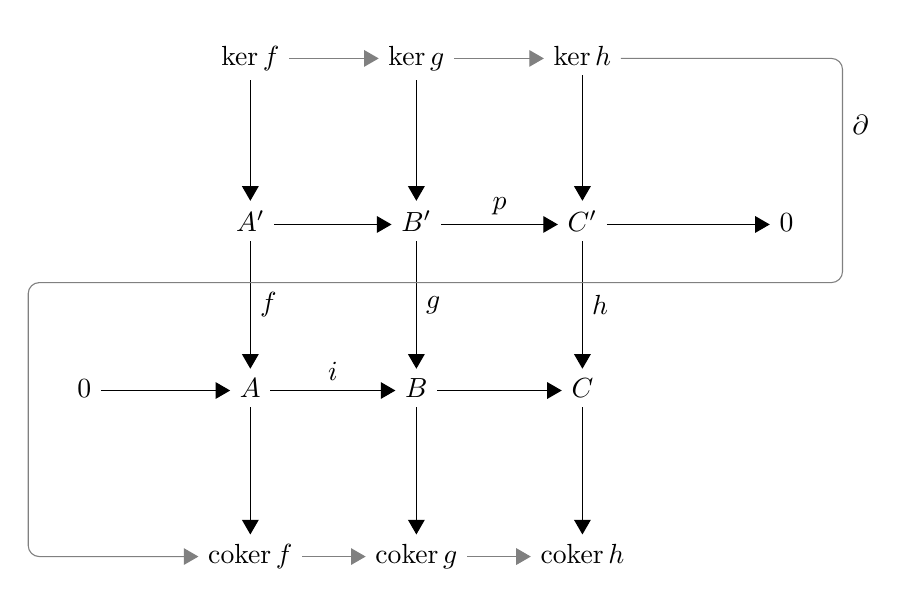
\begin{tikzpicture}[>=triangle 60]
\matrix[matrix of math nodes,column sep={60pt,between origins},row
sep={60pt,between origins},nodes={asymmetrical rectangle}] (s)
{
&|[name=ka]| \ker f &|[name=kb]| \ker g &|[name=kc]| \ker h \\
%
&|[name=A]| A' &|[name=B]| B' &|[name=C]| C' &|[name=01]| 0 \\
%
|[name=02]| 0 &|[name=A']| A &|[name=B']| B &|[name=C']| C \\
%
&|[name=ca]| \coker f &|[name=cb]| \coker g &|[name=cc]| \coker h \\
};
\draw[->] (ka) edge (A)
          (kb) edge (B)
          (kc) edge (C)
          (A) edge (B)
          (B) edge node[auto] {\(p\)} (C)
          (C) edge (01)
          (A) edge node[auto] {\(f\)} (A')
          (B) edge node[auto] {\(g\)} (B')
          (C) edge node[auto] {\(h\)} (C')
          (02) edge (A')
          (A') edge node[auto] {\(i\)} (B')
          (B') edge (C')
          (A') edge (ca)
          (B') edge (cb)
          (C') edge (cc)
;
\draw[->,gray] (ka) edge (kb)
               (kb) edge (kc)
               (ca) edge (cb)
               (cb) edge (cc)
;
\draw[->,gray,rounded corners] (kc) -| node[auto,text=black,pos=.7]
{\(\partial\)} ($(01.east)+(.5,0)$) |- ($(B)!.35!(B')$) -|
($(02.west)+(-.5,0)$) |- (ca);
\end{tikzpicture}

\subsection{8 Term Exact Sequence\label{eightterm}}
This result may be strengthened if the rows are short exact sequences, $0\rightarrow A'\rightarrow B' \rightarrow C' \rightarrow 0$ and \\ $0\rightarrow A\rightarrow B\rightarrow C \rightarrow 0$ to:

$$0 \rightarrow \ker f \rightarrow \ker g \rightarrow \ker h \xrightarrow{\partial} \coker f \rightarrow \coker g\rightarrow \coker h \rightarrow 0,$$

Arising from:

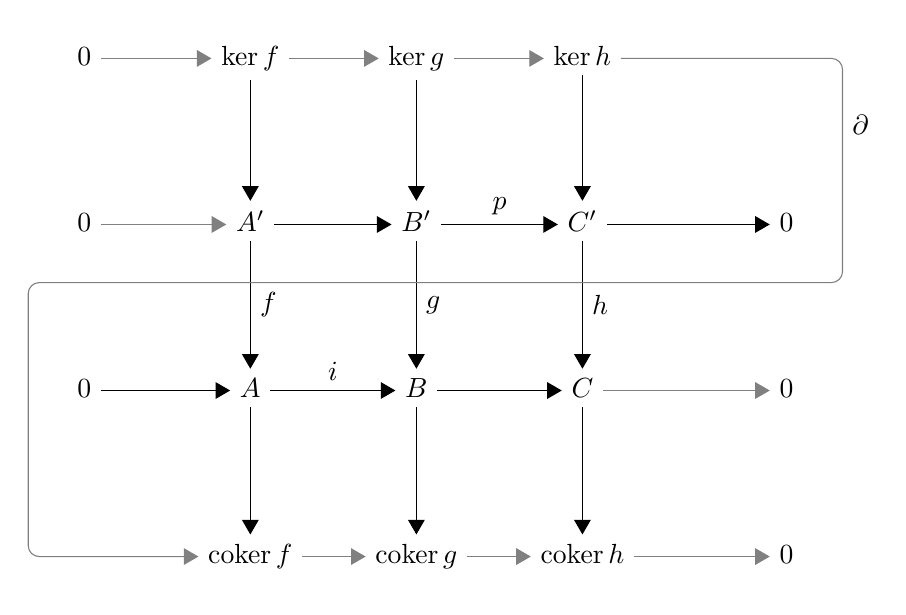
\begin{tikzpicture}[>=triangle 60]
\matrix[matrix of math nodes,column sep={60pt,between origins},row
sep={60pt,between origins},nodes={asymmetrical rectangle}] (s)
{
|[name=kw]| 0  &|[name=ka]| \ker f &|[name=kb]| \ker g &|[name=kc]| \ker h \\
%
|[name=kx]| 0  &|[name=A]| A' &|[name=B]| B' &|[name=C]| C' &|[name=01]| 0 \\
%
|[name=02]| 0 &|[name=A']| A &|[name=B']| B &|[name=C']| C & |[name=ky]| 0 \\
%
&|[name=ca]| \coker f &|[name=cb]| \coker g &|[name=cc]| \coker h & |[name=kz]| 0\\
};
\draw[->] (ka) edge (A)
          (kb) edge (B)
          (kc) edge (C)
          (A) edge (B)
          (B) edge node[auto] {\(p\)} (C)
          (C) edge (01)
          (A) edge node[auto] {\(f\)} (A')
          (B) edge node[auto] {\(g\)} (B')
          (C) edge node[auto] {\(h\)} (C')
          (02) edge (A')
          (A') edge node[auto] {\(i\)} (B')
          (B') edge (C')
          (A') edge (ca)
          (B') edge (cb)
          (C') edge (cc)
;
\draw[->,gray] (ka) edge (kb)
               (kb) edge (kc)
               (ca) edge (cb)
               (cb) edge (cc)
               (kw) edge (ka)
               (kx) edge (A)
               (C') edge (ky)
               (cc) edge (kz)
;
\draw[->,gray,rounded corners] (kc) -| node[auto,text=black,pos=.7]
{\(\partial\)} ($(01.east)+(.5,0)$) |- ($(B)!.35!(B')$) -|
($(02.west)+(-.5,0)$) |- (ca);
\end{tikzpicture}

%%%%%%%%%%%%%%%%%%%%%%%%%%%%%%%%%%%%
\section{Derived Functors of the Inverse Limit}
%%%%%%%%%%%%%%%%%%%%%%%%%%%%%%%%%%%%
We work within the category of Abelian Groups, $\mathbb{Ab}$.

\begin{definition}(Definition of Derived Functors of the Inverse Limit)
Given a tower $\{A_i\}$ in $\mathbb{Ab}$, define the map

$$\Delta:  \prod \{A_i\} \rightarrow \prod \{A_i\}$$
by the element-theoretic formula

$$\Delta(\{a_i\}) \rightarrow (\{ a_i - \text{images of projections}\})$$

In particular, when the indexing set is the Natural numbers, and we have a tower $\{A_i \}: \, \dots \rightarrow A_2 \rightarrow A_1 \rightarrow A_0$. Then,

$$\Delta:  \prod_{i=0}^{\infty} \{A_i\} \rightarrow \prod_{i=0}^{\infty} \{A_i\}$$
by the element-theoretic formula

$$\Delta(\dots, a_i , \dots , a_0 ) = (\dots , a_i - \overline{a_{i+1}},\dots, a_1 - \overline{a_{2}}, a_0 - \overline{a_{1}}  )$$

where $\overline{a_{i+1}}$ denotes the image of $a_{i+1} \in A_{i+1}$ in $A_i$. Clearly, the kernel of $\Delta$ is $\varprojlim A_i$ and we define $\limone A_i$ to be the cockerel of $\Delta$.

\end{definition}

\begin{theorem}(Simplification when Indexed over the Natural Numbers, $\N$\label{simplification})
When the Indexing set is the Natural numbers, $\N$, the higher derived functors vanish (proved by showing it vanishes on enough injectives), and we have definitions of the cohomological derived functor, $\varprojlim^n A_i$:

\begin{eqnarray*}
{\varprojlim}^0 &=& \varprojlim A_i = \text{Ker}\{ \Delta\} \\
{\varprojlim}^1 &=& \text{Coker}\{ \Delta\} \\
{\varprojlim}^n &=& 0 \text{ for } n\neq 0,1.
\end{eqnarray*}

\end{theorem}

\begin{theorem}(A Long Exact Sequence\label{longderivedinv})

If $0\rightarrow \{A_i\} \rightarrow \{B_i\} \rightarrow \{C_i\} \rightarrow 0$, then in this case the Long Exact Sequence of Cohomology follows from applying the Snake Lemma (see \ref{eightterm} ) to

$$\begin{array}{ccccccccc}
0 	&	 \rightarrow &\prod\{A_i\} 	& \rightarrow & \prod\{B_i\} &\rightarrow &\prod\{C_i\} &\rightarrow &0\\
&&\downarrow \Delta&&\downarrow \Delta&&\downarrow \Delta&&\\
0 	&	\rightarrow &\prod\{A_i\} 	& \rightarrow & \prod\{B_i\} &\rightarrow &\prod\{C_i\} &\rightarrow &0\\
\end{array}$$
giving
$$0 \rightarrow \varprojlim\{A_i\} \rightarrow \varprojlim\{B_i\} \rightarrow \varprojlim\{C_i\} \rightarrow  \limone\{A_i\} \rightarrow \limone\{B_i\} \rightarrow \limone\{C_i\} \rightarrow 0$$
\end{theorem}



\begin{example}($lim^1$ of Towers of $p^{th}$-power Factors of the Integers)

Let $A_0 = \Z$ and $A_i = p^i \Z$ be the subgroup generated by $p^i$. We have the exact sequence giving by inclusion/projection which extends to a short exact sequence of towers:

$$0\rightarrow \{p^i \Z \} \rightarrow \{\Z\} \rightarrow \{ \Z / p^i \Z \} \rightarrow 0.$$

The long exact sequence derived from the inverse limit yields

$$ 0 \rightarrow \varprojlim \{p^i \Z \} \rightarrow \varprojlim \{\Z\} \rightarrow \varprojlim \{ \Z / p^i \Z \} \rightarrow \limone \{p^i \Z \} \rightarrow \limone \{\Z\} \rightarrow \limone \{ \Z / p^i \Z \}\rightarrow 0.$$

The groups ${p^i \Z}$ map by inclusion, so the inverse limit reduces to the intersection: $\cap  \{p^i \Z \} = 0$. The identity map connects the trivial tower $\{\Z\}$, hence $\varprojlim \{\Z\} = \Z$, and there is no cokernel so $\limone \{\Z\} = \Z$.  This gives,

$$ 0 \rightarrow 0 \rightarrow \Z \rightarrow \ZP \rightarrow \limone \{p^i \Z \} \rightarrow 0 \rightarrow \limone \{ \Z / p^i \Z \}\rightarrow 0.$$

Hence,

$$ \limone \{p^i \Z \} \cong \ZP / \Z, \text{ and } \limone \{ \Z / p^i \Z \} =0$$
\end{example}


\begin{example}($lim^1$ of Towers of Augmentation Ideals\label{3.2.5})

Similarly, we may consider the filtration of the Iwasawa Algebra by the augmentation ideals:

$$0\rightarrow \{ I_n\}  \rightarrow \{\ZP[G] \}  \rightarrow \{ \ZP [G/G_n]\}  \rightarrow 0$$

This yields 

$$ \limone \{I_n \} \cong \Lambda_G / \ZP[G], \text{ and } \limone  \{ \ZP [G/G_n] \} = 0$$

\end {example}

\begin{proposition}(Interpretation of $lim^1$ in terms of Cohomology Functor, $Ext$)

Let $X$ be $1$-projection in the tower of Carteisan modules.
We may view $lim^1$ explicitly as a derived cohomology functor, by considering $\Z$ as the trivial 
$\Z [X]$-modules, then applying to a Caretian product, $A = \{ A_i \}$:

$$\limone (A) = Ext^1_{\Z[X]} (\Z, A)$$
\end{proposition}

\begin{proof}
The trivial $\Z[x]$-module has a free resolution  $0 \rightarrow \Z[X] \xrightarrow{*(i-X)} \Z[X] \rightarrow \Z \rightarrow 0.$, and the functors agree at degree zero (inverse limit), hence on all higher derived functors. Moreover, this gives a more natural interpretation of why Higher Derived Functors vanish (because the projective resolution vanishes after just two terms).
\end{proof}

\begin{example}(Interpretations of $lim^1$ in Terms of Lifts\label{lifts})

I introduce here a different way to think of $\limone$, these ideas are developed in \ref{mlifts}.

We may think of elements in $\limone \cong Coker \, \Delta \cong Coker \, (i-X)$ as coming from an inability to lift all elements under $(i-X)$, or in other words find a value in the pre-image $(i-X)$.

If $t = (i-X)s$ then $s\in Im \Delta$ and so $s\equiv 0$ in $Coker \Delta$. We may write $s="(i-X)^{-1}"\, t$.

It is an interesting question to unite this idea with basic analysis and the two ways in which the power series of $\frac{1}{1-X}$ may converge using Geometric Progressions:

\begin{eqnarray*}
\frac{1}{1-X}	&=&�1+X+X^2+X^3 + \dots ,\text{ converges when } X^n \rightarrow 0 \\
			&=&�-(\frac 1X+\frac 1{X^2}+\frac 1{X^3} + \dots ),\text{ converges when } \frac1{X^n} \rightarrow 0 \\
\end{eqnarray*} 

I now explain how we may use these techniques when trying to construct a non-zero element in \\
$\limone HH_1(\ZP[G/G_n])$, or equivalently when trying to give an element in $Z(\ZP[G/G_n]^{\otimes 2})$ which cannot be lifted within the kernel (can always lift into $\ZP[G/G_n]^{\otimes 2}$).
\end{example}

\begin{example}(False Tate Curve\label{FTC})

My standard source of examples for illustrating non-commutative pro-$p$ groups is the semi-direct product of two copies of $\ZP$ known as the False Tate Curve, $G \cong \ZP \ltimes \ZP$, where the twisting is by the cyclotomic character ($\rho : \ZP \rightarrow \ZP^*, \, n \rightarrow (1+p)^n$). The FTC enjoys the property of not having any commutative subgroups of finite index. We may think of $G$ as being generated by $a$ and $b$ which each generate a copy of $\ZP$ but which don't commute - rather, $ba = a^{(1+p)} b$. Using this idea we may reduce any element of $G$ to $a^m. b^n$.

We may give the group law more formally as 

\begin{eqnarray}
\nonumber G &=& \ZP  \rtimes \ZP\\
\nonumber     &=& \{(f,h)| (f,h).(f',h') = (f+\rho(h).f', h+h')\}
\end{eqnarray}

Thus $(f,h)^{-1} = (-\rho(-h).f, -h)$, and we denote the \textbf{topological generators of $G$ as $a=(1,0)$ and $b=(0,1)$}.



\end{example}
%%%%%%%%%%%%%%%%%%%%%%%%%%%%%%%%%%%%
\section{Constructing Non-Liftable Elements in $\prod HH_1(\ZP[G/G_n])$}
In this section I describe the process we went through in trying to
construct an element which could not be lifted in the homology.
Equivalently, thinking of complexes we were seeking an element in $ \prod
Z ( \ZP[G/G_n] \otimes \ZP[G/G_n])$ which when lifted (we can always lift
to $ \prod ( \ZP[G/G_n] \otimes \ZP[G/G_n])$ ) was no longer in the kernel
of the boundary map.

Using the FTC, with generators $a,b$, the key is that $[a,b] \in G_2
\setminus G_3$, and more generally using $\phi$ to denote the Frobenius
map, we may increase the exact level of commutivity:

$$[\phi^m(a),\phi^n(b)] \in G_{2+a+b} \setminus G_{3+a+b}$$


\subsection{Infinite Support - Only Interested In The Tail}

\subsection{Products May Become Trivial When We Project}

\subsection{Being Able To Lift The Projection, $p$, Ensures Ee Can Lift
Under $\Delta$}

\subsection{Projection And Lifting Do Not Commute}

\subsection{Element Which Is Not Simple After a Finite Number of Projections}

\subsection{Using a Sum}
%%%%%%%%%%%%%%%%%%%%%%%%%%%%%%%%%%%%
\section{Mittag-Leffler Condition}
%%%%%%%%%%%%%%%%%%%%%%%%%%%%%%%%%%%%
\begin{definition}(Mittag-Leffler Condition\label{ML})

A tower $\{A_i\}$ of abelian groups satisfies the Mittag-Leffler condition if for each $k$ there exists a $j\geq k$ such that the image of $A_i \rightarrow A_k$ equals the image of $A_j \rightarrow A_k$ for all $i\geq j$
\end{definition}

The images of the higher levels in the tower to level $k$ always form a filtration of $A_k$. What we are saying here is that filtration has a finite number of steps at each level (the images of $A_i$ in $A_k$ satisfy the defending chain condition).

Clearly, this will be the case if all the maps $A_{i+1} \rightarrow A_i$ in the tower are onto. If the tower consists of finite abelian groups then each filtration must be finite and so Mittag-Leffler holds. 


\begin{proposition} (see \cite{Weibel}, 3.5.7, Mittag-Leffler Vanishing)

If $\{ A_i \}$ satisfies the Mittag-Leffler condition, then
$$\limone A_i = 0.$$
\end{proposition}

\begin{proof}
We say that $\{A_i\}$ satisfies the trivial Mittag-Leffler condition if for each $k$ there exists $j > k$ such that the map $A_j \rightarrow A_k$ is zero.

Using this idea, if $\{A_i\}$ satisfies the trivial Mittag-Leffler condition, and $b_i \in A_i$ are given we show how to lift. Set $a_k = b_k + {\overline b}_{k+1} + \dots + {\overline b}_{j-1}$, where ${\overline b}_i$ denotes the image of $b_i$ in $A_k$. (Note that ${\overline b}_i =0$ for $i \geq j$.

Then $\Delta$ maps $(\dots, a_1, a_0 ) $ to $(\dots, b_1 , b_0 )$. Thus $\Delta$ is onto and $\limone A_i = 0$ when $\{A_i\}$ satisfies the trivial Mittag-Leffler condition. 

In the general case, let $B_k \subseteq A_k$ be the image of $A_i \rightarrow A_k$ for large $i$. The maps $B_{k+1} \rightarrow B_k$ are all onto, so $\limone B_k = 0$. The tower $\{ A_k / B_k \}$ satisfies the trivial Mittag-Leffler condition, so from above $\limone A_k / B_k = 0$. Considering the short exact sequence of towers,

$$ 0 \rightarrow \{B_i\} \rightarrow \{A_i \} \rightarrow \{A_i / B_i \} \rightarrow 0 $$

we see that $\limone A_i =0$ as required.
\end{proof}

%%%
\begin{corollary} (Vanishing of lim1 for finite towers)

If $\{A_i\}$ is a tower of finite abelian groups, or a tower of finite-dimensional vector spaces over a field, then  $$\limone A_i =0.$$
\end{corollary}
\begin{proof}
This is immediate once one observes that since each level is finite, the images of the higher levels forming a filtration at level $k$ can only have a finite number of steps, satisfying the DCC, hence satisfies Mittag-Leffler.
\end{proof}
%%%
\begin{theorem} (see \cite{scho}, 3.4, $lim^1$ is Cotorsion)

For any inverse sequence $\{G_i \}$, the group 

$$\limone G_i$$
is a cotorsion group.
\end{theorem}

\begin{proof}
Consider 
$$\Delta: \prod_i G_i \rightarrow \prod_i G_i$$

It is easy to see that 
$$\bigoplus_i G_i \subseteq Im(\Delta)$$

and hence there is an exact sequence
$$\frac{\prod_i G_i}{\bigoplus G_i} \rightarrow \limone G_i \rightarrow 0.$$

Now the group $\frac{\prod_i G_i}{\bigoplus G_i}$ is algebraically compact for any choice of $\{G_i\}$ , hence cotorsion, and and quotient of a cotorsion group is again cotorsion.
\end{proof}

\begin{theorem} (see \cite{gray}, Equivalence of Mittag-Leffler and Vaniching of lim1 for Countable Towers)

Suppose given an inverse sequence $\{G_i\}$ with each $G_i$ finite or countable, Then the group 
$$\limone G_i$$
either is zero or uncountable.
\end{theorem}
\begin{proof}
The proof uses the failure of M-L to abstractly construct a set of uncountable elements which give a contradiction.
\end{proof}


\begin{example}(Example of Vanishing of lim1 for the False Tate Curve)
\end{example}
.

.

.

.
\newpage

\begin{example}(Interpretation of the Mittag-Leffler Condition in Terms of Lifting \label{mllifts})

Here I develop the ideas introduced in \ref{lifts}.



%%%%%%%%%%%%%%%%%%%%%%%%%%%%%%%
\section{The Snake Lemma - lim1 Calculation}
%%%%%%%%%%%%%%%%%%%%%%%%%%%%%%%

\begin{theorem} (see \cite{Weibel}, 3.5.8, Homology and Mittag-Leffler\label{3.5.8})

Let $\dots \rightarrow C_1 \rightarrow C_0$ be a tower of chain complexes of abelian groups satisfying the Mittag-Leffler condition, and set $C=\varprojlim C_i$. Then there is an exact sequence for each $q$:

$$0\rightarrow \limone H_{q+1} (C_i) \rightarrow H_q(C) \rightarrow \varprojlim H_q(C_i) \rightarrow 0.$$

\end{theorem}

\begin{proof}
Let $B_i\subset Z_i\subset C_i$ be the sub complexes of boundaries and cycles in the complex $C_i$, so that $Z_i/B_i$ is the chain complex $H_\star (C_i)$ with zero differentials.

Applying the snake lemma to $0\rightarrow \{Z_i\} \rightarrow \{C_i \} \xrightarrow{d} \{C_i [-1]\}$ gives $0\rightarrow \varprojlim Z_i \rightarrow C \rightarrow\dots$ showing that $\varprojlim Z_i$ is a subcomplex of cycles in $C$.

Let $B$ denote the subcomplex $d(C)[1]= (C/Z)[1]$ of boundaries in $C$, so that $Z/B$ is the chain complex $H_\star (C)$ with zero differentials. From the exact sequence of towers
$$0\rightarrow \{Z_i \} \rightarrow \{C_i\} \xrightarrow{d} \{B_i[-1]\} \rightarrow 0$$

We get the long exact sequence,
$$0\rightarrow \varprojlim Z_i \rightarrow \varprojlim C_i \xrightarrow{d} \varprojlim B_i [-1] \rightarrow \limone Z_i \rightarrow \limone C_i \rightarrow \limone B_i[-1] \rightarrow 0$$

Since the $C_i$s satisfy Mittag-Leffler the first derived functor of the inverse limit vanishes: $\limone C_i = 0$, thus

$$0\rightarrow \varprojlim Z_i \rightarrow \varprojlim C_i \xrightarrow{d} \varprojlim B_i [-1] \rightarrow \limone Z_i \rightarrow 0\rightarrow \limone B_i[-1] \rightarrow 0$$

Sandwiched, $\limone B_i[-1]=0$, and translating $\limone B_i=0$. 

We also have that $0\rightarrow \varprojlim Z_i \rightarrow \varprojlim C_i \xrightarrow{d} \varprojlim B_i [-1] \rightarrow \limone Z_i \rightarrow 0$. 

On the left hand side of the exact sequence we may replace $\varprojlim C_i  / \varprojlim Z_i $ by $B[-1]$ giving exact sequence, 

$$ 0\rightarrow B[-1] \rightarrow \varprojlim B_i [-1] \rightarrow \limone Z_i$$

Similarly, the short exact sequence of towers, $0\rightarrow \{ B_i \} \rightarrow \{ Z_i \} \rightarrow H_\star (C_i) \rightarrow 0$ yields

$$0\rightarrow \varprojlim B_i \rightarrow Z \rightarrow \varprojlim H_\star(C_i) \rightarrow 0 \rightarrow \limone Z_i \rightarrow \limone H_\star  (C_i)\rightarrow 0$$

Hence, $\limone Z_i \cong \limone H_\star  (C_i)$ and $0\rightarrow \varprojlim B_i \rightarrow Z \rightarrow \varprojlim H_\star(C_i) \rightarrow 0$ is exact.

Finally $C$ has the filtration by sub complexes

$$0\subset B \subset \varprojlim B_i \subset Z \subset C.$$

From above the filtration quotients are $B$, $\limone Z_i[+1] = \limone H_\star(C_i)[+1], \varprojlim H_\star (C_i)$, and $C/Z$ respectively. By definition, $H_*(C) = Z/B$, and the theorem follows.
\end{proof}

\subsection{The Snake Lemma - lim1 and Homology}

As a corollary to \ref{3.5.8} Weibel then applies this formula for complete complexes to yield the following.
%%%
\begin{theorem} (see \cite{Weibel}, 5.5.5, Eilenberg-Moore Filtration Sequence for complete complexes)

Suppose that $C$ is complete with respect to a filtration by subcomplexes. Associated to the tower $\{C/F_p C\}$ is the sequence of \ref{3.5.8}:

$$0\rightarrow \limone H_{n+1} (C/F_pC) \rightarrow H_n(C) \xrightarrow{\pi} \varprojlim H_n(C/F_pC) \rightarrow 0.$$

\end{theorem}

From this we can see that the finite quotients of Hochschild Homolgy, as an homology theory can also be calculated in this way:

\begin{corollary} (Eilenberg-Moore Filtration Sequence applied to Hochischild Homology of Finite Quotients)
Let G be a uniform pro-$p$ group, where $G_n$ denotes the subgroup of $p^{n-1}$st powers. Denote the Iwasawa Algebra, $\varprojlim \ZP [G/G_n]$ by $\Lambda_G$, then:
$$0\rightarrow \limone HH_{n+1} (\ZP[G/G_n]) \rightarrow HH_n(\Lambda_G) \rightarrow \varprojlim HH_n (\ZP[G/G_n]) \rightarrow 0.$$
 
\end{corollary}
%%%

%%%

\subsection{Eilenberg-Moore Filtration Sequence}

We had been discussing how to combine the cohomology theory of the higher derived functors of the inverse limit (the invariants under left shift), and the homology theory of bimodules. The issue being that the cohomology groups had negative homological degree, and so the classical picture of composed functors, following Grothendieck did not quite work. We introduced the idea that if the inverse limit is indexed over $\mathbb{N}$ then only the inverse limit, and $\underleftarrow{\text{lim}^1}$ (measuring how far from being surjective the projection maps between layers are) are needed with the higher derived functors vanishing. And felt that the inverse limit of $HH_1$s should have the $HH_1$ of the Iwasawa algebra, and the $\underleftarrow{\text{lim}^1}$ term of the $HH_2$s featuring.


\begin{theorem}(see \cite{Weibel}, 5.5.5, Eilenberg-Moore Filtration Sequence for complete complexes\label{emsequences})

{Suppose that $C$ is complete with respect to a filtration by subcomplexes. Associated to the tower $C/F_p C$ is the exact sequence:}

$$0 \rightarrow  \underleftarrow{\text{lim}^1} H_{n+1}(C/F_pC) \rightarrow H_n(C) \rightarrow  \underleftarrow{\text{lim}}\,H_n(C/F_pC) \rightarrow 0.$$ 

This sequence is associated to the filtration on $H_*(C)$ as follows. The left hand term $\underleftarrow{\text{lim}^1} H_{n+1}(C/F_pC)$ is $\cap F_pH_n(C)$, and the right-hand term is the Hausdorff quotient of $H_*(C)$:

$$H_*(C)/\cap F_pH_n(C) \cong \underleftarrow{\text{lim}} H_n(C) / F_pH_n(C) \cong \underleftarrow{\text{lim}} H_n(C/F_pC).$$

\end{theorem}

\begin{proof}

Taking the inverse limit of the exact sequences of towers 

$$0 \rightarrow \{ F_pH_*(C) \} \rightarrow H_*(C) \rightarrow \{ H_*(C) / F_pH*(C) \} \rightarrow 0$$

$$0 \rightarrow \{ H_*(C) / F_pH_*(C) \} \rightarrow \{ H_*(C/F_pC) \}$$

shows that $H_*(C) / F_p H_*(C)$ is a sub object of $\underleftarrow{\text{lim}} H_*(C) / F_pH_*(C)$, which is in turn a subobject of 

$\underleftarrow{\text{lim}} H_n(C/F_pC)$. Now combine this with the standard behaviour of  $\underleftarrow{\text{lim}^1}$.

\end{proof}



\chapter{Hochschild Homology}
In this chapter I discuss the homology of bi-modules known as Hochschild Homology. I begin with an opaque definition via complexes before re-interpreting in terms of more natural objects. I then use Shapiro's lemma to decompose this homology theory in the case of group rings, into a direct sum over conjugacy classes, and show how this is just group homology in disguise.
%%%%%%%%%%%%%%%%%%%%%%%%%%%%%%%%%%%%
\section{Definition of Hochschild Homology}
%%%%%%%%%%%%%%%%%%%%%%%%%%%%%%%%%%%%
\subsection{Intuition}
Hochschild Homology is an homology theory (for some interpretation of �homology theory�) of $S$-$S$-bimodules for a ring $S$.

Whenever one has a $S$-$S$-bimodule, one can think of this just as well as $S\otimes S$-module (here I�m using that $S$ is commutative, but for non-commutative rings not so much changes). And for any commutative ring $S$, there is an obvious map $S\otimes S\to S$ called �multiplication.�

The extension of scalars by this ring homomorphism (which is just the annoying commutative algebra way of saying the tensor product $M\otimes_{S\otimes S}S$ is what people seem to insist on calling �coinvariants� (making that word a very overloaded operator in this field). This no help in picking a name to say for it, but the best written notation for me is the somewhat suggestive $HH_0$.

Another way to think of this functor $HH_0(M)$ is as the largest quotient of $M$ on which the left and right actions coincide.

Hochschild homology is what happens when we take this extension of scalars in the only proper way to do anything in homological algebra: in the derived sense.

The main point is that you should take the tensor product above and replace one (or both) of its factors with a projective resolution. You then have a complex in place of your tensor product, and the extension of the short exact sequence to have right exactness gives the Hochschild homology groups $HH_i(M)$ as the homology of this complex. We recover $HH_0$ as the $0^{th}$ homology of this complex.

The definition given in books is based on one particular resolution of $S$ as an $S\otimes S$-bimodule. This is ugly and hard to use for many purposes, but is completely general. It works for every ring. But polynomial rings are much nicer than just any old ring. In particular, they have a much smaller resolution as bimodules over themselves, called the Koszul resolution. This has the distinct advantage of being finite rank over $S\otimes S$, and of finite length (in fact, its length is the number of variables of $S$), neither of which are true of the more general resolution (in fact, for many rings, there is no upper bound on the $i$ for which $HH_i$ might be non-zero. In polynomial rings, we know that the number of variables gives an upper bound).

So, we can calculate $HH_*(M)$ by simply tensoring with this complex, but this is not as nice as we might hope, since taking the homology of a complex whose terms are complicated modules is hard, even if the differentials are very explicit. This may be good enough for a computer, for people, it�s a bit dissatisfying.

But as I mentioned before, you can resolve either side, and is useful for some purposes to do one, and for the purposes the other. For example, if one is lucky and can find a nice resolution of the module one is Hochschild homologizing, then tensoring with $S$, one has a complex whose terms are free modules over $S$ and whose differentials are easy to calculate from those of the original complex (just hit the matrices of the map with the multiplication map).

If one is really lucky, then this complex will have trivial differentials after extension of scalars. This sounds like too much ask, I suppose, but in fact this is true for any modules whose Hochschild homology is free (for example, for Soergel bimodules in type A, by results of Jake Rasmussen).

So, why do we care? Well, if we have a category of bimodules over $S$ which is closed under tensor product, then $HH_*$ functions as a categorical trace: We have an isomorphism $HH_*(A\otimes B)\cong HH_*(B\otimes A)$ (as vector spaces, not necessarily as  $S$ modules). It turns out that if you apply this to the category of Soergel bimodules (a categorification of the Hecke algebra), then you get back a categorification of the Jones-Ocneanu trace on the Hecke algebra.

\subsection{Formal Definition}
\begin{definition}(See \cite{rosenberg}, 6.1.1, \textbf{Definition of Hochschild Homology}\label{hochschildcomplex})

Let $k$ be a commutative ring and let $R$ be a $k$-algebra. 

We write $R^{\otimes n}$ for 
$$R\otimes_k R \otimes_k \dots \otimes_k R \,(n \text{ times}).$$
The Hochschild homology of $R$ is by definition the homology $HH_* (R)$ of the Hochschild Complex

$$C_*(R): \, \dots \xrightarrow{b_{n+2}} R^{\otimes{n+2}} \xrightarrow{b_{n+1}}R^{\otimes{n+1}} \xrightarrow{b_{n}}R^{\otimes{n}} \xrightarrow{b_{n-1}}\dots \xrightarrow{b_{1}} R,$$
where $R^{\otimes{n+1}}$ occurs in degree $n$ and the boundary map $b$ is the $k$-linear map defined by the formula 
$$b_n(a_0 \otimes a_1 \otimes \dots \otimes a_n) = b'_n(a_0\otimes a_1\otimes \dots \otimes a_n ) + (-1)^n(a_n a_0 \otimes a_1 \otimes \dots \otimes a_{n-1},$$

where

$$b'_n(a_0\otimes a_1\otimes \dots \otimes a_n ) = \sum_{i=0}^{n-1} (-1)^i a_0 \otimes \dots \otimes a_i a_{i+1} \otimes \dots \otimes a_n).$$
\end{definition}

Since the differential is $k$-linear, $HH_i (R)$ is a $k$-module for each $i$ (though not usually an $R$-module). It is useful to note, however, that if $R$ is commutative, $b'$ and $b$ commute with multiplication by $R$ on the left, so $HH_i(R)$ is an $R$-module.

We can make this ad-hoc definition seem more natural (and is sometimes given as the definition) by observing the following:

\begin{proposition}(See \cite{rosenberg}, 6.1.4, \textbf{Presenting Hochschild Homology as a Tor Group})

Let $k$ be a commutative ring and let $R$ be a $k$-algebra which is projective as a module over $k$ (automatic if $k$ is a field). The Hochschild homology $HH_*(R)$ is just $Tor_*^{R\otimes_k R^{op}} (R,R)$, where $R^{op}$ denoted $R$ with multiplication reversed, and we identify two-sided $R$-modules with left of right modules for $R\otimes_k R^{op}$.
\end{proposition}

\begin{proof}

This arises from identifying the sequence as the Acyclic Resolution of the ring $R$ as $R\otimes R^{op}$-modules tensored with $R$, see \cite{benson}, 2.11.
\end{proof}

More generally, for an $R$-$R$-bimodule, $A$, we can define the Hocschild Homolgy, $HH_n(A,R)$ via the above complex, where at each level we replace the final copy of $R$ in the tensor string with a copy of $A$.

Equivalently, we can seine as a $Tor$ Group:

$$HH_n(A,R) = Tor_n^{R\otimes_kR^{op}} (A,R)$$

From this definition we recover the case A=R, and have the notation:

$$HH_n(R) \equiv HH_n(R,R).$$

\section{Decomposition of Hochschild Homology for Group Rings}

\begin{theorem}(see \cite{benson}, 2.11.2, \textbf{Splitting up Hochschild Homology over Conjugacy Classes}\label{splitting})

The additive structure of the Hochschild Homology of a group algebra $RG$ is given by
$$HH_n (RG) \cong \bigoplus_{g\in ccl(G)} H_n(Z_G(g),R), \,\forall \, n\geq 0$$
where $Z_G(g)$ denotes the centraliser of the element $g$ in the group $G$.

\end{theorem}

\begin{proof}
We have the natural expression, 
$$HH_n(RG) \cong Tor^{RG \otimes RG^{op}}_n (RG,RG^*)$$

Now $RG^{op} \cong RG$, via $g \rightarrow g^{-1}$, and $RG\otimes RG \cong R(G \times G)$. The $R(G\otimes G)$-module structure on $RG$ is given by the two-sided action
$$(g_1, g_2) : g \rightarrow g_1 g g_2^{-1},$$
and so it is just the permutation module (induced module), $R_{\Delta(G)} \uparrow^{G\times G}$ on the cosets of the diagonal group
$$\Delta (G) = \{ (g,g) \vert g\in G \} \subseteq G \times G.$$

Similarly, $RG^*$ is the conduced module $R_{\Delta(G)} \Uparrow^{G\times G}$. So by the Eckmann-Shapiro Lemma, \ref{shapiro}, we have
\begin{eqnarray*}
HH_n(RG) 	&\cong& Tor_n^{R(G\times G)} (R_{\Delta(G)} \uparrow^{G\times G} , R_{\Delta(G)} \Uparrow^{G\times G})\\
		 	&\cong& Tor_n^{R \Delta (G)} (R_{\Delta(G)} , R_{\Delta(G)} \Uparrow^{G\times G}\downarrow_{\Delta(G)}).
\end{eqnarray*}			
By the Mackey Decomposition Theorem (see \ref{mackey}),

$$\left(R_{\Delta(G)} , R_{\Delta(G)} \Uparrow^{G\times G}\downarrow_{\Delta(G)}\right) \cong \prod_{g \in ccl(G)} R_{\Delta(Z(g))}\Uparrow^{\Delta(G)}$$

and so by another application of the Eckmann-Shapiro Lemmma we obtain

\begin{eqnarray*}
HH_n(RG) &\cong& \prod_{g \in ccl(G)} Tor^{RG}_n (R, R_{Z(g)}\Uparrow^G)\\
                  &\cong& \prod_{g \in ccl(G)} Tor^{RZ(g)}_n(R,R)\\ 
                  &\cong& \prod_{g \in ccl(G)} H_n(Z(g), R). 
\end{eqnarray*}
\end{proof}

Moreover, an element in $a_0\otimes a_1\otimes \dots \otimes a_n \in R^{\otimes n+1}$ gives rise to a contribution in the conjugacy class of $(\prod a_n)$. The element $(\prod a_n)$ is known as the marker of $a_0\otimes a_1\otimes \dots \otimes a_n$ and it is easily seen to be preserved under boundary maps.

In particular when we focus on integral group rings:

\begin{corollary}(See \cite{Weibel}, 9.7.5, \textbf{Decomposition of Hochschild Homology over Conjugacy Classes\label{decomposition}})

The Hochschild Homology of a group ring has a natural decomposition into a direct sum indexed by conjugacy classes of the group. Denoting the centraliser of an element $g$ in the group $G$ by $Z(g)$, and writing $H_n(G;A)$ for the group homology of $G$ with coefficients in $A$ we have:

$$HH_n (\Z[G]) = \bigoplus_{g\in \text{ccl} (G)} H_n(Z(g); \Z), \, \forall \, n\geq 0$$
\end{corollary}



\begin{corollary}(Hochschild Homology of Low Degree for Group Rings\label{lowdeg})

Using results on terms of Group Homology of low degree, see \ref{lowdeggroup}, we may specialise \ref{decomposition} above to give:
\begin{eqnarray*}
HH_0 (\Z[G]) 	&\cong& 		\bigoplus_{g\in \text{ccl} (G)} H_0(Z(g); \Z) \\
			&\cong& \bigoplus_{g\in \text{ccl} (G)} \Z\\
HH_1 (\Z[G]) 	&\cong& 		\bigoplus_{g\in \text{ccl} (G)} H_1(Z(g); \Z) \\
			&\cong& \bigoplus_{g\in \text{ccl} (G)} Z(g)^{ab}
\end{eqnarray*}
\end{corollary}

%%%%%%%%%%%%%%%%%%%%%%%%%%%%%%%

\section{Notation for Elements in $HH_1 (\Z [G])$\label{notation}}

From above,
\begin{eqnarray*}
HH_1(\Z[G]) 	&\cong& \text{Ker }b_1 / \text{Im }b_2 \\
			&\cong& \text{Ker }b: \{\Z G \otimes \Z G \rightarrow \Z G \} /
\text{Im }b: \{ \Z G \otimes \Z G \otimes \Z G \rightarrow \Z G \otimes
\Z G \}\\
			&\cong& \bigoplus_{g\in \text{ccl} (G)} Z(g)^{ab}.
\end{eqnarray*}

Chasing elements through the splitting proof above, \ref{splitting}, the
marker of the element $a\otimes b \in \Z G \otimes \Z G$, $ab\in G$, gives
the conjugacy class which this element contributes to.

Moreover, by working in the quotient, $\text{Ker }b_1 / \text{Im }b_2$ we
may reduce to the case $b\in Z(ab)$, or equivalently $b\in Z(a)$.

For $a,b \in G$, the representative $a\otimes b$ of an element in $HH_1(\Z
[G])$ may be thought of as an element $b$ centralising $ab$, written as a
component,

$$ \begin{array}{c} a\\ \big\vert \\ ab\\ \end{array} \in \bigoplus_{g\in
\text{ccl} (G)} Z(g)^{ab}.$$


\chapter{Completions}
I begin this chapter by working with the projective resolutions of the group ring to show finiteness of integral group homology. I then apply this to the decomposition of Hochschild homology and show that the Mittag-Leffler condition holds. I use the vanishing of $lim^1$ to comment on the connection between the homology of the completed resolution and the completion of the homologies of the finite resolution.

I then interpret these results in terms of cofinal sequences, and for the $n=1$ explain the connection with the Lie Bracket.

Finally, I introduce the concept of a free product and explain how our result has implications for the topology here.


%%%%%%%%%%%%%%%%%%%%%%%%%%%%%%%%%%%%
\section{Finiteness}
%%%%%%%%%%%%%%%%%%%%%%%%%%%%%%%%%%%%

In order to calculate the group homology via $Tor$ groups we use a canonical resolutions $B_\star$ and $B_\star^u$ of the trivial $G$-module $\Z$ by free left $\Z G$-modules.

\begin{definition} (\textbf{The \textit{Normalised} and \textit{Unnormalised} Bar Resolutions \label{bar}})

$$0\leftarrow \Z \xleftarrow{\epsilon}B_0\xleftarrow{d} B_1\xleftarrow{d} B_2 \xleftarrow{d} \dots .$$

$$0\leftarrow \Z \xleftarrow{\epsilon}B_0^u\xleftarrow{d} B_1^u\xleftarrow{d} B_2^u \xleftarrow{d} \dots .$$

Where $B_0^u$ is $\Z G$. Let the symbol $[\,]$ denote $1 \in \Z G$, and $\epsilon: B_0^u \rightarrow \Z$ the map which sends $[\,]$ to $1$.

For $n\geq 1$, $B_n^u$ is the free $\Z G$-module on the set of all symbols $[ g_1 \otimes \dots \otimes g_n]$ with $g_i \in G$, while $B_n$ is the free $\Z G$-module on the (smaller) set of all symbols $[ g_1 | \dots | g_n ]$ with the $g_i \in G - \{1 \}$.

\end{definition}

We may identify $B_n$ with the quotient $B_n^u$ by the submodule $S_n$ generated by the set of all \\ symbols $[g_1 \otimes \dots \otimes g_n]$ with some $g_i$ equal to $1$.

\begin{definition} (\textbf{Differentials in normalised and unnormalised resolutions})

For $n\geq 1$, define the differential $d: B_n^u \rightarrow B_{n-1}^u$ to be $d = \sum_{i=0}^n (-1)^i d_i$, where:
\begin{eqnarray}
d_0([g_1\otimes\dots\otimes g_n]) &=& g_1 [g_2 \otimes \dots \otimes g_n]; \nonumber\\
d_i([g_1\otimes\dots\otimes g_n]) &=& [g_1 \otimes \dots \otimes g_i g_{i+1} \otimes \dots \otimes g_n]\text{ for } i=1, \dots, n-1;\nonumber\\
d_n([g_1\otimes\dots\otimes g_n]) &=& [g_1 \otimes \dots \otimes g_{n-1}].\nonumber
\end{eqnarray}

Similarly, the differential for $B_\star$ is given by the following:
$$d_i([g_1|\dots|g_n]) = [[g_1|\dots|g_i g_{i+1} | \dots |g_n ] \text{ when }g_ig_{i+1}\neq 1, \text{ and } =0\text{ when } g_ig_{i+1}=1.$$
\end{definition}

\begin{theorem} (\textbf{Bar resolutions})
The sequences in \ref{bar} above are exact. Thus both $B_\star$ and $B_\star^u$ are resolutions of $\Z$ by free left $\Z G$-modules.
\end{theorem}

\begin{example}(\textbf{First Group Homology with Coefficients in Integers})

For every right $G$-module $A$, $H_\star (G;A)$ is the homology of the chain complex $A\otimes_{\Z G} B_\star$. In particular we see that $H_1(G; \Z)$ is the free abelian group on the symbols $[g], \, g\in G$, with the relations $[1]=0$, and $[f]+[g] = [fg]$ for ll $f,g\in G$. This recovers the calculation earlier that 

$$H_1(G; \Z ) = G/ [G,G].$$

\end{example}

%%%
\begin{theorem} (see \cite{Weibel}, 6.5.8, \textbf{(Co)Homology Groups are Torsion})

Let $G$ be a finite group with $m$ elements. Then for $n \neq 0$ and every $G$-module $A$, both $H_n(G;A)$ and $H^n(G;A)$ are annihilated by $m$, that is they are $\Z /m$-modules.

\end{theorem} 


6.5.8

\begin{proof}

Let $\eta$ denote the endomorphism of $B_*$, which is multiplication by
$(m-N)$ on $B_0$ and multiplication by $m$ on $B-n$, $\neq 0$. We claim
that $\eta$ is null homotopic. So applying $A\otimes$ or $Hom( - , A)$,
will then yield a null homotopic map, which must become zero upon taking
homology, proving the above theorem.

For definitions of "null homotopic" and "chain contraction" refer to \ref{df1.2.3}.

Define $\nu_n : B_n \rightarrow B_{n+1}$ by the formula

$$ \nu_V([g_1 | \dots | g_n ]) = (-1)^{n+1} \sum_{g\in G} [ g_1 | \dots
|g_n |g].$$

Setting $\omega = [g_1 | \dots |g_n])$ and $\epsilon = (-1)^{n+1}$, we
compute for $n\neq 0$

$$d\nu_n(\omega) = \epsilon \sum \{ g_1[\dots | g] + \sum (-1)^i [\dots
|g_i g_{i+1}| \dots | g] - \epsilon [\dots | g_{n-1} | g_n g] + \epsilon
\omega \}$$

$$\nu_{n-1} d (\omega) = - \epsilon \sum \{ g_1[\dots | g] + \sum (-1)^i
[\dots |g_i g_{i+1}| \dots | g] - \epsilon [\dots | g_{n-1} | g] \}.$$

As the sums over all $g \in G$ of $[\dots | g_n g ]$ and $[\dots | g]$
agree, we see that $(dv+vd)(\omega)$ is $\epsilon^2 \sum \omega =
m\omega$. Now $d\nu_0([]) = d(-\sum [g]) = 9m-N){}$, where $N = \sum g$ is
the norm. Thus $\{ \nu_V \}$ provides the chain contraction needed to make
$\nu$ null homotopic.

\end{proof}


%%%


%%%
\begin{corollary} (see \cite{Weibel}, 6.5.10, \textbf{Finitely generated modules give finite (Co)Homology groups}\label{6.5.10})

If $G$ is a finite group and $A$ is a finitely generated $G$-module, then $H_n(G;A)$ and $H^n(G;A)$ are finite abelian groups for all $n\neq 0$.

\end{corollary}

\begin{proof}
Each $A \otimes_{\Z G} B_n$ and $Hom_G(B_n , A)$ is a finitely generated
abelian group. Hence $H_n(G;A)$ and $H^n(G;A)$ are finitely generated $\Z
/ m$-modules when $n\neq 0$, hence finite.
\end{proof}

In particular for a finite group $G$ and $A = \Z$, the integral homology groups $H_n(G;\Z)$ are finite for $n \geq 1$. 

\section{Complete Resolution for Calculating the Hochschild Homology of an Iwasawa Algebra}

%%%%%%%%%%%%%%%%%%%%%%%%%%%%%%%%%%%%%%%%%%%%%%
I now present a filtration on the Hochschild Complex of the group algebra, $\ZP[G]$, see \ref{hochschildcomplex}, so that the quotients $C_{\ZP[G]} / F_p C_{\ZP[G]}$ recover the Hoschschild Complex for finite quotients, $C_{\ZP[G/G_n]}$. 

Taking the completion, $\varprojlim C_{\ZP[G]} / F_p C_{\ZP [G]} \cong \varprojlim C_{\ZP[G/G_n]}$ gives the complex for the Iwasawa Algebra, $\Lambda_G$, where the tensor in the original complex is now replaced with a completed tensor, see \ref{completedtensor}.

At level $0$, the filtration of $C_0 = \ZP[G]$, is given by $F_p C_0 = I_p$, the $p^{th}$ Augmentation Ideal, where (see \ref{3.2.5}),

$$ C_0 / F_p C_0 \cong \ZP [G/G_n].$$

At level $1$, the filtration of $C_1 = \ZP[G] \otimes \ZP[G]$, is given by $F_p C_1 = I_p \otimes \ZP[G] + \ZP[G] \otimes I_p$ where,

\begin{eqnarray*}
C_1 / F_p C_1 &\cong& (\ZP[G] \otimes \ZP[G]) / ( I_p \otimes \ZP[G] + \ZP[G] \otimes I_p)\\
				&\cong& (\ZP[G] \otimes \ZP[G/G_n]) / ( I_p \otimes \ZP[G/G_n])\\
				&\cong& (\ZP[G/G_n] \otimes \ZP[G/G_n]).
\end{eqnarray*}

\begin{proposition}(Structure of Completed Complex)

The Hochschild Complex, $\{C_n\}$, of the group algebra $\ZP[G]$ possesses a filtration $\{F_pC\}$ where
\begin{eqnarray*}
F_p C_n 	&\cong& I_p \otimes \ZP[G]^{\otimes n} + \text{ symmetric rearrangements}\\
		&\cong& \sum_{i=0}^n \ZP[G]^{\otimes i} \otimes I_p \otimes \ZP[G]^{\otimes n-i}
\end{eqnarray*}

Moreover, these filtrations are preserved under the boundary map, $b$, since $I_p$ is an ideal. Hence maps on Quotients,

$$C_{\ZP[G]} / F_p C_{\ZP[G]} \cong C_{\ZP[G/G_n]},$$

are well defined and we may form the inverse limit, 

$$\varprojlim C_{\ZP[G]} / F_p C_{\ZP [G]} \cong \varprojlim C_{\ZP[G/G_n]}$$

which then gives the Hochschild Complex for the Iwasawa Algebra, $\Lambda_G$, where the tensor in the original complex is now replaced with a completed tensor.
\end{proposition}

In particular, if we take $C$ to be the chain of simplicial modules used to calculate Hochschild Homology of the group ring of $G$, $F_nC$ be the image for the group of $p^n$-th powers, then we have the Iwasawa Algebra appearing as the completion of $C/F_nC$:

$$0 \rightarrow  \underleftarrow{\text{lim}^1} HH_{n+1}(\Z_p[G/G^m]) \rightarrow HH_n(\Lambda_G) \rightarrow  \underleftarrow{\text{lim}}\,H_n(\Z_p[G/G^m]) \rightarrow 0.$$ 

Specialising for $n = 0,1$:

$$0 \rightarrow  \underleftarrow{\text{lim}^1} HH_{1}(\Z_p[G/G^m]) \rightarrow HH_0(\Lambda_G) \rightarrow  \underleftarrow{\text{lim}}\,H_0(\Z_p[G/G^m]) \rightarrow 0.$$ 

$$0 \rightarrow  \underleftarrow{\text{lim}^1} HH_{2}(\Z_p[G/G^m]) \rightarrow HH_1(\Lambda_G) \rightarrow  \underleftarrow{\text{lim}}\,H_1(\Z_p[G/G^m]) \rightarrow 0.$$ 

Giving,

$$ \underleftarrow{\text{lim}}\,H_0(\Z_p[G/G^m]) =    HH_0(\Lambda_G) / \underleftarrow{\text{lim}^1} HH_{1}(\Z_p[G/G^m])$$

Which might tie in the work by Mahesh where he looks into different presentations of $\Z_p [Conj(G)]$ using traces.

$$ \underleftarrow{\text{lim}}\,H_1(\Z_p[G/G^m]) =    HH_1(\Lambda_G) / \underleftarrow{\text{lim}^1} HH_{2}(\Z_p[G/G^m])$$

%%%%%%%%%%%%%%%%%%%%%%%%%%%%%%%%%%%%%%%%%%%%%%
\begin{proposition}(Direct Proof of E-M Sequence for Hochschild Homology)

$$0 \rightarrow  \underleftarrow{\text{lim}^1} HH_{1}(\Z_p[G/G^m]) \rightarrow HH_0(\Lambda_G) \rightarrow  \underleftarrow{\text{lim}}\,H_0(\Z_p[G/G^m]) \rightarrow 0.$$ 
\end{proposition}

\begin{proof}
Taking $\Delta = i - \text{Projection}$, we have the onto maps, with kernels the inverse limits for each $n\in \mathbb{N}$:

$$0\rightarrow \varprojlim \ZP[G/G_n]^{\otimes 2} \rightarrow \prod \ZP[G/G_n]^{\otimes 2} \xrightarrow{\Delta}  \prod \ZP[G/G_n]^{\otimes 2} \rightarrow 0$$

and,

$$0\rightarrow \varprojlim \ZP[G/G_n] \rightarrow \prod \ZP[G/G_n] \xrightarrow{\Delta}  \prod \ZP[G/G_n]\rightarrow 0.$$

We may connect these sequences using the extension of the Lie algebra commutator map, $d$. By the definition of homology we have the following diagram using the snake lemma construction (see \ref{eightterm}), and denoting the kernel of a map by$Z(-)$:


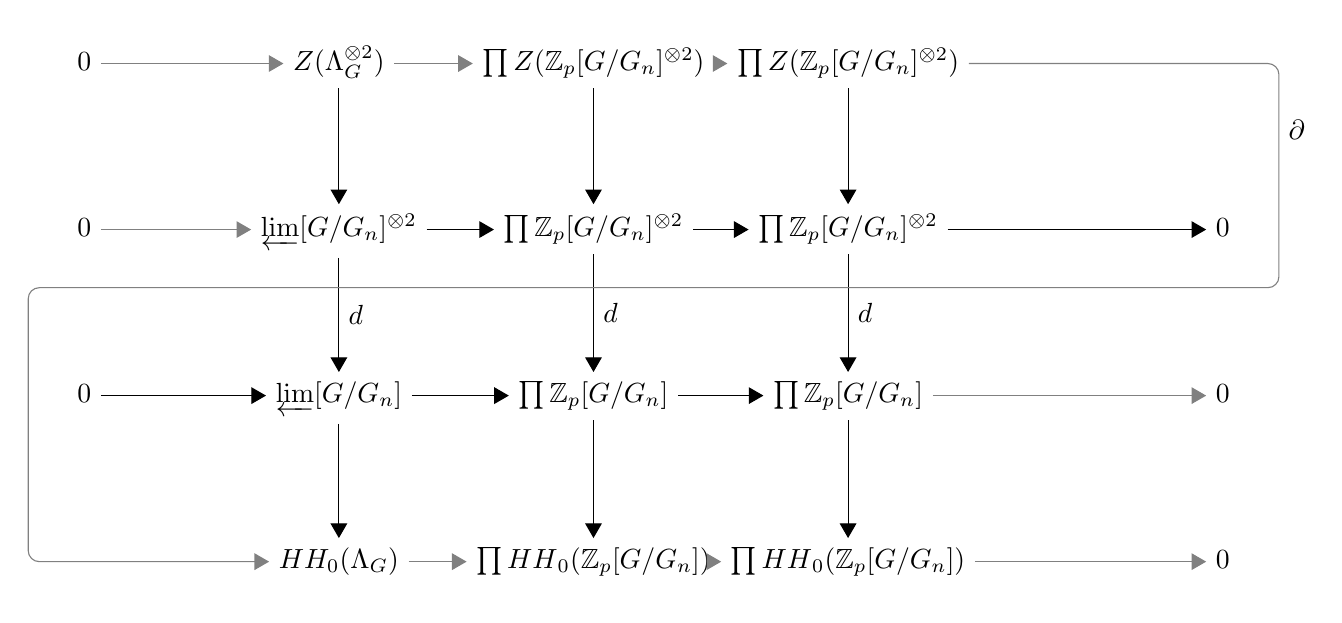
\begin{tikzpicture}[>=triangle 60]
\matrix[matrix of math nodes,column sep={92pt,between origins},row
sep={60pt,between origins},nodes={asymmetrical rectangle}] (s)
{
|[name=kw]| 0  &|[name=ka]| Z(\Lambda_G^{\otimes 2}) &|[name=kb]| \prod Z(\ZP[G/G_n]^{\otimes 2}) &|[name=kc]| \prod Z(\ZP[G/G_n]^{\otimes 2}) \\
%
|[name=kx]| 0  &|[name=A]| \varprojlim[G/G_n]^{\otimes 2} &|[name=B]| \prod \ZP [G/G_n]^{\otimes 2} &|[name=C]| \prod \ZP [G/G_n]^{\otimes 2}  &|[name=01]| 0 \\
%
|[name=02]| 0 &|[name=A']| \varprojlim[G/G_n] &|[name=B']| \prod \ZP [G/G_n] &|[name=C']| \prod \ZP [G/G_n] & |[name=ky]| 0 \\
%
&|[name=ca]| HH_0 (\Lambda_G) &|[name=cb]| \prod {HH}_0 (\ZP [G/G_n]) &|[name=cc]| \prod {HH}_0 (\ZP [G/G_n]) & |[name=kz]| 0\\
};
\draw[->] (ka) edge (A)
          (kb) edge (B)
          (kc) edge (C)
          (A) edge (B)
          (B) edge (C)
          (C) edge (01)
          (A) edge node[auto] {\(d\)} (A')
          (B) edge node[auto] {\(d\)} (B')
          (C) edge node[auto] {\(d\)} (C')
          (02) edge (A')
          (A') edge  (B')
          (B') edge (C')
          (A') edge (ca)
          (B') edge (cb)
          (C') edge (cc)
;
\draw[->,gray] (ka) edge (kb)
               (kb) edge (kc)
               (ca) edge (cb)
               (cb) edge (cc)
               (kw) edge (ka)
               (kx) edge (A)
               (C') edge (ky)
               (cc) edge (kz)
;
\draw[->,gray,rounded corners] (kc) -| node[auto,text=black,pos=.7]
{\(\partial\)} ($(01.east)+(.5,0)$) |- ($(B)!.35!(B')$) -|
($(02.west)+(-.5,0)$) |- (ca);
\end{tikzpicture}

Hence, the snake lemma gives:

$$\prod Z(\ZP [G/G_n]^{\otimes 2} ) \xrightarrow{\Delta} \prod Z(\ZP [G/G_n]^{\otimes 2} ) \xrightarrow {\partial} HH_0 (\Lambda_G) \rightarrow \prod HH_0 (\ZP [G/G_n] ) \xrightarrow{\Delta} \prod HH_0 (\ZP [G/G_n] ) \rightarrow 0$$

By definition of the inverse limit we also have the exact sequence:

$$0\rightarrow \varprojlim HH_0 (\ZP[G/G_n]) \rightarrow \prod HH_0 (\ZP [G/G_n] ) \xrightarrow{\Delta} \prod HH_0 (\ZP [G/G_n] ) \rightarrow 0$$

Hence,
\begin{eqnarray}
Ker\, \Delta 	&\cong& \varprojlim HH_0 (\ZP[G/G_n]) \\
			&\cong& HH_0(\Lambda_G) / Im(\partial) \\
			&\cong& HH_0(\Lambda_G) / Coker ( \Delta) \\
			&\cong& HH_0(\Lambda_G) / \limone (Z(\ZP[G/G_n]^{\otimes 2}))
\end{eqnarray}

Referring to the proof of \ref{3.5.8} I recall that if we denote $B_i \subset Z_i \subset C_i$ to be the sub complexes of boundaries and cycles in the complex $C_i$, then $Z_i/B_i$ is the chain complex $H_*(C_i)$, and by sandwiching, $\limone Z_i \cong \limone H_*(C_i)$. This gives  $\limone (Z(\ZP[G/G_n]^{\otimes 2})) \cong \limone HH_1(\ZP[G/G_n])$. Hence, 
$$\varprojlim HH_0 (\ZP[G/G_n]) \cong HH_0(\Lambda_G) / \limone (HH_1(\ZP[G/G_n])),$$
or equivalently,
$$0\rightarrow  \limone (HH_1(\ZP[G/G_n])) \rightarrow HH_0(\Lambda_G) \rightarrow \varprojlim HH_0 (\ZP[G/G_n])\rightarrow 0.$$


\end{proof}
%%%%%%%%%%%%%%%%%%%%%%%%%%%%%%%%%%%%%%%%%%%%%%


The finiteness result, \ref{6.5.10} applies when G is the centraliser of an element the finite quotient of an uniform pro-$p$ group, and combining \ref{decomposition} with \ref{emsequences} we get:

\begin{corollary}(\textbf{Completions and Hochschild Homology}\label{finitehh})
\begin{enumerate}
\item By finiteness, the Mittag-Leffler condition applies giving:
$$\limone HH_m (\ZP [G/G_n]) = \limone \left \{ \bigoplus _{g_n \in \text{ccl } G/G_n } H_m (Z(g_n); \Z) \right \} = 0, \forall\, m\geq 1$$

\item Hence, \ref{emsequences} reduces to:

$$ 0 \rightarrow 0 \rightarrow HH_m \left ( \varprojlim_n \ZP [G/G_n] \right )  \rightarrow  \varprojlim_n \left ( HH_m ( \ZP [G/G_n])\right ) \rightarrow 0, \forall m\geq 0$$

We may write in terms of the Iwasawa Algebra, $\Lambda_G$:

$$HH_m (\Lambda_G) \cong  \varprojlim_n (HH_m ( \ZP [G/G_n]), \forall m\geq 0.$$
 
\end{enumerate}
\end{corollary}

\begin{example} (Intuition for the Approach of this Chapter)


Our intuition for this was built up in several stages:

To begin with we realised that the acts of taking homology and taking inverse limits need not commute, and we thought that we might be able to combine the derived functors of taking the inverse limit with the derived functors of homology (Hoschschild Homology in this case) to construct a term of total degree 1. Thus the first level might consist of the zeroth level of the inverse limit with the first level of the homology and vice versa.

Things then looked a lot more difficult when we realised that since the Inverse Limit was defined as the set of Invaraints (under shift map $\Delta$), it gave rise to a homology theory and so the higher derived functors had negative homological degree. This meant that the level of total degree 1 might consist of first homology with zeroth inverse limit, second homology and first derived functor of the inverse limit, third homology and second derived functor of the inverse limit... .

This situation was simplified by the idea that when the indexing set is the natural numbers, all the higher derived functors of the inverse limit vanish ($\varprojlim^n A_i = 0$ for all $n\geq 2$, see \ref{simplification}). So we were left to combe the inverse limit of $HH_n$ and the first derived functor of the inverse limit applied to $HH_{n+1}$. This is precisely how we use the Eilenberg-Moore Filtration, see \ref{emsequences}.
  
\end{example}
%%%

%%%%%%%%%%%%%%%%%%%%%%%%%%%%%%%%%%%%
\section{Cofinal Completions}
\newpage


%%%%%%%%%%%%%%%%%%%%%%%%%%%%%%%%%%%%

%%%%%%%%%%%%%%%%%%%%%%%%%%%%%%%%%%%%
\section{Interpreting as Commutivity of Inverse Limits and Lie Commutator Bracket}

Let $G$ be a Uniform pro-$p$ group, and $G_n$ the Frobenius powers, let $d$ be the commutator map used in associative Lie algebras: $d(a \otimes b ) \equiv ab - ba$, and denote the Iwasawa algebra, $\varprojlim \ZP [G/G_n]$, by $\Lambda_G$.


\begin{proposition}($lim^1$: Comparing Inverse Limits and Lie Bracket)
\begin{eqnarray*}
\limone HH_1 (\ZP [G/G_n]) &\cong& \varprojlim \{d \{\ZP[G/G_n] \otimes \ZP[G/G_n] \}\} / d \{ \varprojlim \{\ZP[G/G_n] \otimes \ZP[G/G_n] \}\} \\
					&\cong& \varprojlim \{d \{\ZP[G/G_n] \otimes \ZP[G/G_n] \}\} / d \{ \Lambda_G \widehat{\otimes} \Lambda_G \} \\
\end{eqnarray*}
\end{proposition}

\begin{proof}

Consider the exact sequence of towers arising from,

$$0 \rightarrow Ker_d(\ZP[G/G_n] \otimes \ZP[G/G_n]) \rightarrow (\ZP[G/G_n] \otimes \ZP[G/G_n])  \xrightarrow{d} d(\ZP[G/G_n] \otimes \ZP[G/G_n])  \rightarrow 0$$

Applying the eight term exact sequence of \ref{longderivedinv} we have:
\begin{eqnarray*}
0 \rightarrow \varprojlim Ker_d(\ZP[G/G_n] \otimes \ZP[G/G_n]) \rightarrow \varprojlim (\ZP[G/G_n] \otimes \ZP[G/G_n])  \xrightarrow{d} \varprojlim d(\ZP[G/G_n] \otimes \ZP[G/G_n])  \rightarrow \dots\\
\dots \rightarrow \limone Ker_d(\ZP[G/G_n] \otimes \ZP[G/G_n]) \rightarrow \limone(\ZP[G/G_n] \otimes \ZP[G/G_n])  \xrightarrow{d}  \limone d(\ZP[G/G_n] \otimes \ZP[G/G_n])  \rightarrow 0
\end{eqnarray*}

Since maps in the tower $\{  \ZP[G/G_n] \otimes  \ZP[G/G_n] \}$ are onto, by \ref{ML} we have that 

$$\limone \{  \ZP[G/G_n] \otimes  \ZP[G/G_n] \} = 0.$$ 

Hence,
\begin{eqnarray*}
0 \rightarrow \varprojlim Ker_d(\ZP[G/G_n] \otimes \ZP[G/G_n]) \rightarrow \varprojlim (\ZP[G/G_n] \otimes \ZP[G/G_n])  \xrightarrow{d}  \dots\\
\dots \xrightarrow{d} \varprojlim d(\ZP[G/G_n] \otimes \ZP[G/G_n])  \rightarrow \limone Ker_d(\ZP[G/G_n] \otimes \ZP[G/G_n]) \rightarrow 0
\end{eqnarray*}

By exactness,

$$ \limone Ker_d(\ZP[G/G_n] \otimes \ZP[G/G_n]) \cong  \varprojlim d(\ZP[G/G_n] \otimes \ZP[G/G_n])  / d(\varprojlim (\ZP[G/G_n] \otimes \ZP[G/G_n]))$$

The proof of \ref{3.5.8} gives  $\limone HH_1 (\ZP [G/G_n]) \cong  Ker_d(\ZP[G/G_n] \otimes \ZP[G/G_n])$ which yields the result.
\end{proof}

Prior to applying the Mittag-Leffler condition to $\limone HH_1(\ZP [G/G_n])$ I interpreted this in terms of a question about the commutivity of Inverse Limits and Lie Brackets as follows.  

I was interested in finding elements in 
$$\underleftarrow{lim}^1 \, HH_1(\mathbb{Z} _p [G/G_n]).$$
\\
Equivalently, to show $lim^1 \neq 0$, I needed to find an element in

$$\underleftarrow{lim} \,\{d (  \mathbb{Z}_p [G/G_n] \otimes
\mathbb{Z}_p{[G/G_n]} ) \} $$

which was not in

$$d ( \underleftarrow{lim} \,  \{\mathbb{Z}_p{[G/G_n]} \otimes
\mathbb{Z}_p{[G/G_n]} \}) \cong  d \{ \Lambda_G \widehat{\otimes} \Lambda_G \}.$$

From universal properties, 

$$\underleftarrow{lim} \,\{d (  \mathbb{Z}_p{[G/G_n]} \otimes
\mathbb{Z}_p{[G/G_n]} ) \} \rightarrow d ( \underleftarrow{lim} \,
\{\mathbb{Z}_p{[G/G_n]} \otimes
\mathbb{Z}_p{[G/G_n]} \})\rightarrow 0.$$

I hoped that in some interesting cases we would have
$$\underleftarrow{lim} \,\{d (  \mathbb{Z}_p{[G/G_n]} \otimes
\mathbb{Z}_p{[G/G_n]} ) \} \neq d ( \underleftarrow{lim} \,
\{\mathbb{Z}_p{[G/G_n]} \otimes
\mathbb{Z}_p{[G/G_n]} \}).$$

But in \ref{finitehh} above I showed $\limone HH_1 \{\ZP [G/G_n]\} =0$, hence

$$\underleftarrow{lim} \,\{d (  \mathbb{Z}_p{[G/G_n]} \otimes
\mathbb{Z}_p{[G/G_n]} ) \} \,\cong\, d ( \underleftarrow{lim} \,
\{\mathbb{Z}_p{[G/G_n]} \otimes
\mathbb{Z}_p{[G/G_n]} \}).$$


%%%%%%%%%%%%%%%%%%%%%%%%%%%%%%%%%%%%
\section{Interpreting vanishing of lim1 in terms of Hausdorff Property}
%%%%%%%%%%%%%%%%%%%%%%%%%%%%%%%%%%%%
I begin by recalling from \ref{emsequences}) that the term we have shown to be zero, $\limone H_{n+1}(C/F_pC)$ is infact the image of the filtration on homology, $\bigcap F_pH_n(C)$, measuring how far from being Hausdorff the inherited filtration on homology is.

I begin by expressing this for the n=0 case. Since the filtrations on the 1st level of the complex take the form $I_p + \ZP[G]$, we are looking at the images of homology groups $(I_p )/(d(I_p,\ZP[G])$ in $(\ZP[G])/(d(\ZP[G],\ZP[G])$, which is $(I_p+\ZP[G])/(d(\ZP[G],\ZP[G])$, and so we may state (from \ref{finitehh}) that 

$$\bigcap_{p=0}^{\infty} (I_p+\ZP[G])/(d(\ZP[G],\ZP[G])) = 0$$

Equivalently, 

$$\bigcap_{p=0}^{\infty} (I_p+\ZP[G]) =d(\ZP[G],\ZP[G])$$

It is tempting to think that just because our original complex is Hausdorff it's filtration has to be. We may rephrase this as if $\bigcap A_i = 0$, it seems that $\bigcap (A_i + M) = M$, or equivalently $\bigcap (A_i + M)/M = 0$.

This is true for $M$ finite when we can split up the sum into  $\bigcap (A_i /M) + \bigcap (M/M) = 0$, but there can be more interesting behaviour for $M$ infinite. Let $A_i = \prod_{n= - \infty}^{-i} \Z$, and $M = \bigoplus_{n= -\infty}^0\Z$. Then for each $i$, $A_i + M = \prod_{n= - \infty}^{0} \Z$. Hence, 

$$\bigcap (A_i + M)/M =  \left\{ \prod \Z \right\} / \left\{ \bigoplus \Z \right\} = \{\text{Uncountable}\} /\{\text{Countable}\} \neq 0.$$ 



\chapter{Free Products}
%%%%%%%%%%%%%%%%%%%%%%%%%%%%%%%%%%%%
\section{Connection with Free Products}
%%%%%%%%%%%%%%%%%%%%%%%%%%%%%%%%%%%%

I now approach the question of comparing the completed Hochschold Homology of the finite quotients of the group algebra with the Hochschild Homology of the completed group algebra, the content of \ref{finitehh}, from a different angle - of course we must reach the same conclusion that the two are equivalent, but by giving the topology, under which the Hochschild homology of finite sums completes we can have an understanding of what is happening which is not dependent on the choice of a filtration.

Given a family of groups, there are many different ways of combining these to get another group. In this chapter I introduce ideas of Mel'nikov, (see \cite{melnikov}), where he gives the construction $\bigstar G_\lambda$ for groups  $G_{\lambda}$ with $\{ \lambda \in \Lambda \}$, an extension of the free product, over  a not necessarily finite indexing set $\Lambda$. I follow the treatment of \cite{profgps} contained in Chapter 9, and Appendix D (where the product is instead written $\amalg^r G_{\lambda}$).

\section{Cartesian Product}
The \textbf{cartesian} (or unrestricted direct) product,

$$C = \text{Cr}_{\lambda\in\Lambda} G_{\lambda}$$

is the group with underlying set given by the product of the $G_{\lambda}$ as sets - vectors whose $\lambda$-component lies in $G_{\lambda}$, and where the group operation is defined by multiplication of components: $(g_\lambda)(h_\lambda) = (g_\lambda h_\lambda)$ for $g_\lambda, h_\lambda \in G_\lambda$.

The cartesian product may be thought of as a universal construction of a group, $G$:

Define the projections $\pi_\lambda : G \rightarrow G_\lambda$ by taking $\pi_\lambda (x)$ to be the $\lambda$-th component of $x$. $\pi_\lambda$ is a homomorphism for each $\lambda$.

Given a family of homomorphisms $\phi_\lambda: H\rightarrow G_\lambda$ for some group $H$, there exists a unique homomorphism $\phi:H\rightarrow C$ such that $\phi \circ \pi_\lambda = \phi_\lambda$ for all $\lambda$.

The existence of the map $\phi$ gives the following commutative diagram:
$$\begin{array}{ccc}
  H&   &   \\
  \downarrow \phi&  \searrow \phi_\lambda &   \\
  C&  \xrightarrow{\pi_\lambda} & G_\lambda   
\end{array}$$


\section{Direct Product}
The subset of the $(g_\lambda) \in \text{Cr}_{\lambda\in\Lambda} G_{\lambda}$ such that $g_\lambda = i_\lambda$ for almost all $\lambda$, so that the sequence is trivial with finitely many exceptions, is called the \textbf{external direct} product,

$$D = \text{Dr}_{\lambda\in\Lambda} G_{\lambda}$$

The $G_\lambda$ are referred to as the direct factors. $D$ is a normal subgroup of $C$, and equal for a finite indexing set $\Lambda = \{  \lambda_1, \lambda_2, \dots, \lambda_n \}$. The products are then written,

$$D = G_{\lambda_1}\, \times \, G_{\lambda_2} \, \times\, \dots \, \times \, G_{\lambda_n}$$

And should the groups be abelian, then this is usually written additively as:

$$D = G_{\lambda_1}\, \oplus \, G_{\lambda_2}\, \oplus \, \dots \, \oplus  \, G_{\lambda_n}$$

\section{Free Products}

 The \textbf{abstract free product} of the family $G_\lambda$ is a group $G$ together with a collection of homomorphisms $l_\lambda: G_\lambda \rightarrow G$ with universal property  that for another such group $H$ and set of homomorphisms  $\phi_\lambda: G_\lambda \rightarrow H$, there is a unique homomorphism of groups $\phi:G\rightarrow H$ such that $\phi \circ l_\lambda  = \phi_\lambda$, and the following diagram commutes:

$$\begin{array}{ccc}
  G_\lambda& \xrightarrow{l_\lambda}  & G  \\
  \downarrow \phi_\lambda&  \swarrow \phi&   \\
  H&  &   
\end{array}$$

The free product is sometimes denoted $F = \text{Fr}_{\lambda\in\Lambda} G_{\lambda} \text{ or } \Asterisk_{\lambda\in\Lambda} G_{\lambda}$ .

From the category-theoretic viewpoint this free product is a coproduct in the category of groups (the product being the cartesian product defined above).

For each $\lambda$, taking $H = G_\lambda$, and maps $\phi_\lambda = \text{id}$, and with the other $\phi_\mu$ trivial, we see that $\phi\circ l_\lambda = \text{id}\vert _{G_\lambda}$ and so each $l_\lambda$ is injective.

Uniqueness of this construction is clear from the universal property. Existence can be shown using an explicit description on words, where letters are taken from the disjoint union of the $G_\lambda$ (we are only working up to an isomorphism of $G_\lambda$, so may assume they do not intersect), products are by juxtapostion, and the only relations are contracting/ expanding letters lying in the same group $G_\lambda$, and absorbing/inserting identity elements.

If $\Lambda$ is finte, $\Lambda = \{  \lambda_1, \lambda_2, \dots, \lambda_n \}$, it is usual to write product as

$$G_{\lambda_1}\, \Asterisk  \, G_{\lambda_2} \, \Asterisk \, \dots \, \Asterisk \, G_{\lambda_n}$$

The free product has the following properties:
\begin{enumerate}

\item For $\lambda$ finite, there is a natural epimorphism of groups from $\Asterisk_{\lambda\in\Lambda} G_\lambda$ onto $\text{Dr}_{\lambda\in\Lambda} G_\lambda$, defined by taking only the entries in �G_{\lambda}$ in the word of an element in $\Asterisk_{\lambda\in\Lambda} G_\lambda$ , and then fuse together by taking the product. The kernel of this map consists of any elements in $G_{\alpha}$, where $\alpha \neq \lambda$, and such that the product of elements in with index $\lambda$ is trivial, $i_{\lambda} \in G_{\lambda}$.

\item When we take the abelianisation of the free product we may simplify words by sliding elements past each other in the free group to clump together the $G_{\lambda}$, and furthermore by exchanging places within the $G_{\lambda}$ reduces to the abelianisation, $G_{\lambda}^{ab}$, in each component. The group law is now the same as for the Direct Product.

So for abelian families $G_\lambda$, we have $(\Asterisk_{\lambda\in\Lambda} G_\lambda)_\text{ab} \cong \text{Dr}_{\lambda\in\Lambda} G_\lambda$. For a finite index we have:

$$(\Asterisk_{\lambda\in\Lambda} G_\lambda )^{\text{ab}} \cong \bigoplus_{\lambda\in\Lambda} G_\lambda$$


\item In general, 
$$\left (\Asterisk_{\lambda\in\Lambda} G_\lambda\right )^{\text{ab}} \, \cong \, \text{Dr}_{\lambda\in\Lambda} (G_\lambda^{\text{ab}}).$$
\end{enumerate}

\section{Products of Profinite Groups}

Following Melnikov, see \cite{melnikov}, I explain how the topology of profinte groups and spaces can be used to control what is happening in the inverse limits of such products, and how such products may themselves be represented as products.

I will discuss $p$-groups and pro-$p$ groups in this section although the same ideas could be applied to $\mathcal C$ and pro-$\mathcal C$ groups for $\mathcal C$ any full class of finite groups (meaning it is closed under subgroups, homomorphic images and group extensions).

\subsection{When the Indexing Family is Finite\label{extend}}

Following \cite{profgps}, Chapter 9. Let $G_i$ for $(i=1,\dots, n)$ be a finite collection of pro-$p$ groups. A free pro-$p$ product of these groups consists of a pro-$p$ group $G$ and continuous homomorphisms $\phi_i : G_i \rightarrow G$, for $i = 1,\dots , n$ satisfying the following universal property:

$$\begin{array}{ccc}
  G &   &   \\
  \uparrow \phi_i &  \searrow \psi&   \\
  G_i& \xrightarrow{\psi_i} & K   
\end{array}$$

for any pro-$p$ group K and any continuous homomorphisms $\psi_i : G_i \rightarrow K$, $i=1, \dots , n$, there is a unique homomorphism induced by the $\psi_i$, and we refer to the $\phi_i$ as the canonical maps of the free pro-$p$ product.

We denote a free pro-$p$ product of the groups $G_1, \dots , G_n$ by

$$G =  \amalg_{i=1}^n G_i \text{ or by } G = G_1\amalg \dots \amalg G_n.$

This universal property needs only be tested for finite $p$-groups $K$, as it then holds automatically for any pro-$p$ group $K$, since $K$ is an inverse limit of $p$-groups.

We need the following properties,

\begin{proposition}{(see \cite{profgps}, 9.1, Properties of the Free pro-$\mathcal C$ Product)}

\begin{enumerate}
\item Let $\{ G_i \vert i= 1, \dots , n\}$ be a collection of pro-$p$ groups. Then there exists a unique free pro-$p$ product
$$G = \amalg_{i=1}^n G_i.$$

\item Let $G^{abs} = G_1 \Asterisk \dots \Asterisk G_n$ be a free product of $G_1, \dots G_n$ considered as abstract groups. Denote by $\phi_i^{abs} : G_i \rightarrow G^{abs}$ the natural embeddings. Let 

\vsapce
\vsapce


\boxed{$$\mathcal N = \left \{ N \lhd_f G^{abs} \vert (\phi_i^{abs})^{-1} (N) \lhd_o G_i \text{ for all } i = 1, \dots , n \text{ and } G^{abs} / N \in \mathcal C\right \}$$}

\vspace
\vsapce

Then $\mathcal N$ is filtered from below, and we may take $G = \mathcal K_{\mathcal N} (G^{abs})$ to be the completion of $G^{abs}$ with respect to the topology determined by $\mathcal N$. Denote by $l:G^{abs} \rightarrow G$ the natural homomorphism and put $\phi_i = l \circ \phi_i^{abs}$, then each $\phi_i$ is continuous and $G$ together with these maps satisfies the universal property.

\item Let $G = A \Asterisk B$ be a free product of abstract groups. Then denoting the pro-$p$ completion of a group $G$ by $G_{\hat{p}$,  
$$G_{\hat{p}} = A_{\hat{p}} \amalg B_{\hat{p}}.$$

\item Let $G_1, \dots , G_n$ be pro-$\mathcal C$ groups and let $G = G_1 \amalg \dots \amalg G_n$ be their free pro-$\mathcal C$ product.
Then, the natural homomorphisms 
$$\phi_j: G_j \rightarrow G = \amalg_{i=1}^n G_i\,\, (j=1,\dots , n)$$
are monomorphisms; and $G = \overline{<\phi_i(G_i) \vert i = 1, \dots , n>}$

\textbf{Thus we may think of the $G_i$ as being embedded in $G^{abs} = G_1 \Asterisk \dots \Asterisk G_n$. Then $G = G_1 \amalg \dots \amalg G_n$ is the completion of $G^{abs}$ with respect to the topology defined by the collection of all normal subgroups $N$ of findte index in $G^{abs}$ such that $N\cap G_i$ is open in $G_i$, $(i=1, \dots, n)$ and the quotient, $G^{abs}
/ N$ is a pro-$p$ group.}
\end{enumerate}

\end{proposition}

The key point of this completed construction is that it now commutes with taking inverse limits:

\begin{proposition}{(see \cite{profgps}, 9.1.7, Inverse Limits and Free Pro-$\mathcal C$ Products Commute\label{commutes})}


Let $\{G_{1i}, \mu_{1ij}, I_1\}$ and $\{G_{2i} , \mu_{2ij}, I_2 \}$ be surjective inverse systems of pro-$p$ groups over posets $I_1$ and $I_2$, respectively. Then,

\begin{itemize}

\item $I_1 \times I_2$ is a poset in a natural way and $\{G_{1i} \amalg G_{2k} , \mu_{1ij} \amalg \mu_{2kr}, I_1 \times I_2 \}$ is an inverse system over $I_1\times I_2$.

\item In this setup Inverse Limits and Free Pro-$p$ Products Commute: 
$$\left(\varprojlim_{I_1} G_{1i} \right ) \amalg \left (\varprojlim_{I_2} G_{2i} \right) \cong \varprojlim_{I_1\times I_2} \left (G_{1i} \amalg G_{2k} \right). $$
\end{itemize}
\end{proposition}

\begin{proposition}{(see \cite{profgps}, 9.1.8, Monomorphism in Completion)}

Let $G_1, \dots , G_n$ be pro-$p$ groups. Let $G^{abs} = G_1 \Asterisk \dots \Asterisk G_n$ be the abstract free product of the groups. The the natural homomorphism,

$$l: G^{abs} = G_1 \Asterisk \dots \Asterisk G_n \rightarrow G = G_1 \amalg \dots \amalg G_n$

is a monomorphism.
\end{proposition}

\subsection{When the indexing family is a profinite space}

This requires a more general concept of "free pro-$p$ product" than the one used in \ref{extend}, above.

Let $ G$ be a pro-$p$ group and let $\{G_{\alpha} \vert \alpha \in A \}$ be a collection of pro-$p$ groups indexed by a set $A$. For each $\alpha \in A$, let $l_\alpha : G_\alpha \rightarrow G$ be a continuous homomorphism. One says that the family $\{ l_\alpha \vert \alpha \in A\}$ is \textbf{convergent} if whenever $U$ is an open neighbourhood of $1$ in $G$, then $U$ contains all but a finite number of the images $l_\alpha (G_\alpha)$. We say that $G$ together with the $l_\alpha$ is the free pro-$p$ product of the groups $G_\alpha$ if the following universal property is satisfied: whenever $\{ \lambda_\alpha : G_\alpha \rightarrow K \vert \alpha \in A \}$ is a convergent family of continuous homomorphisms into a pro-$p$ group $K$, then there exists a unique continuous homomorphism $\lambda: G \rightarrow K$ such that 

$$\begin{array}{ccc}
  G_\alpha & \xrightarrow{l_\alpha}  & G  \\
   & \lambda_\alpha \searrow & \downarrow \lambda  \\
  & & K   
\end{array}$$


commutes, for all $\alpha \in A$. One easily sees that if such a free product exists, then the maps $l_\alpha$ are injections.

 
\begin{proposition}{(see \cite{profgps}, D.3.1, Construction of the Free pro-$\mathcal C$ Product)\label{comphoch}}
The free pro-$\mathcal C$ product exists, and is denoted by
$$G = \amalg_{\alpha \in A}^r G_\alpha .$$
To construct the pro-$\mathcal C$ product one proceeds as follows:
\begin{itemize}
\item Let $G^{abs} = \Asterisk_{\alpha\in A} G_\alpa$ be the free product of the $G_\alpha$ as abstract groups (so with finite support).
\item Consider the pro-$\mathcal C$ topology on $G^{abs}$ determined by the collection of normal subgroups $N$ of finite index in $G^{abs}$ such that $G^{abs}/ N \in \mathcal C, \, N \cap G_\alpha$ is open in $G_\alpha$, for each $\alpha \in A$, and $N\geq G_\alpha$, for all but finitely many $\alpha$.
\item Put $$G = \varprojlim_N G/N.$$
\item Then $G$ together with the maps $l_\alpha : G_\alpha \rightarrow G$ is the free pro-$\mathcal C$ product $ \amalg_{\alpha \in A}^r G_\alpha .$
\item If the set $A$ is finite, the "convergence" property of the homomorphisms $l_\alpha$ is automatic; in that case, instead of $\amalg^r$, we use the symbol $\amalg$ as in \ref{extend}.
\item As in \ref{commutes}, this extended free pro-$\mathcal C$ product commutes with taking inverse limits, and this is the key application.
\end{itemize} 
\end{propostion}

\section{Completions of the Hoschschild Homology}
I follow the construction of \ref{comphoch} to describe the topology giving the completion. 

Since abelianization and inverse limits commute,  the abelianization of the inverse limit, $G = \varprojlim_N G^{abs}/N$, is the same as the inverse limit of the abelianisations, $(G^{abs}/N)^{ab}$. 

Passing to the abelianization simplifies the quotients in the inverse limits. In the finite quotient, for $N$ of finite index in $G^{abs}$ with $G^{abs}/ N$ pro-$p$, and $N \cap G_\alpha$ open in $G_\alpha$, for each $\alpha \in A$, and $N\geq G_\alpha$, for all but finitely many $\alpha$.

$$\left(G^{abs}/N\right )^{ab} \cong \left(\Asterisk_ {\alpha \in Ccl (G)} H_\alpha / N\right)^{ab} \cong \left ( \bigoplus_ {\alpha \in Ccl (G)} {H_\alpha}^{ab} \right) / M$$ 
where $H_{\alpha}$ is the component of homology in the decomposition over conjugacy classes. Since $H_{\alpha}$ is already abelian we have 

$$(G^{abs}/N)^{ab} \cong \left( \bigoplus_ {\alpha \in Ccl (G)} {H_\alpha} \right) / M$$

Where the component of $M$ in each summand is of finite index in $H_\alpha$, and moreover the component is equal in all but finitely many $\alpha$. We thus see that the abelianisation of the free product is a completion of the direct sum.

\subsection{Case n=0}

Following, \ref{lowdeg}, the components $H_\alpha$ in each conjugacy class are copies of $\ZP$.

\subsection{Case n=1}

Similarly, the components $H_\alpha$ in each conjugacy class are the abelianisations of the Centralisers of Conjugacy Class representatives, $Z(\alpha)$. More generally, we have the $n$-th group homology with trivial coefficients appearing here.

This may be summarised as,

\begin{eqnarray}
\nonumber \varprojlim_n HH_1 (\ZP[G/G_n]) &=& \varprojlim_n \,\, \bigoplus_{g_n\in \text{ccl }G/G_n} Z(g G_n)^{ab}\\
\nonumber						&=& \varprojlim_n \left[ \Asterisk_{g\in \text{ccl }G/G_n} Z(g G_n) \right]^{ab}\\		\nonumber						&=& \left[ \varprojlim_n  \Asterisk_{g\in \text{ccl }G/G_n} Z(g G_n) \right]^{ab}\\		\nonumber						&=& \left[ \amalg_{g \in \text{ccl }G}^r Z(g) \right]^{ab}\\
\nonumber						&=& \left[ \varprojlim_{\mathcal N} (\Asterisk_{g \in \text{ccl }G} Z(g))/N\right]^{ab}\\
\nonumber						&=& \varprojlim_{\mathcal N} \left[ (\Asterisk_{g \in \text{ccl }G} Z(g))/N\right]^{ab}\\
\nonumber						&=& \varprojlim_{\mathcal M} \bigoplus_{g \in \text{ccl }G} Z(g)^{ab}/M
\end{eqnarray}

Where we have a clear description of the subgroups of the direct sum, $\mathcal M$. 

This explains why the inverse limit of the Hochschild Homologies on the finite is just a completion of $HH_1(\ZP [G])$.

Finally, I need to explain why $HH_1 (\Lambda(G))$ yields the same thing. This is clear when we compute the Hochschild Homology of the Iwasawa Algebra by replacing the usual tensor product formulation with completed tensor products.

%%%%%%%%%%%%%%%%%%%%%%%%%%%%%%%%%%%%%%%%%%%%%%%%%%%%%%%%%%%%
\section{Conjugacy Classes of the False Tate Curve}
%%%%%%%%%%%%%%%%%%%%%%%%%%%%%%%%%%%%%%%%%%%%%%%%%%%%%%%%%%%%
Now that we can work with the full pro-$p$ and take a completion, knowing the structure of conjugacy classes and centralisers is important.

We study the semi-direct product of $2$ copies of $\ZP$,

\begin{eqnarray}
\nonumber G		&=&		F \rtimes H\\
				&=&		\{ (f,h). (f' , h') = (f+\rho(h) f' , h+h')\}
\end{eqnarray}

Where $\rho : n \rightarrow (1+p)^n$.

Hence, 

$$ (f,h)^{-1} = (-\rho(-h) f , -h)$$

Notice, $\rho(\ZP) = (1+p)^{\ZP} = 1+p \ZP$.

$$(a,b)^{(g,h)} = (\rho(-h)(a+(\rho(b)-1_g_,b)$$

As we vary over all possible pairs $g$ and $h$:

$$(a,b)^{(g,h)} =  ((1+p \ZP)(a+(1-\rho(b))\ZP), b)$$

Since $val(\rho(b) - 1) = val(b)+1 = val (bp)

$$(a,b)^{(g,h)} =  ((1+p \ZP)(a+bp\ZP), b)$$

ie

$$ccl(a,b) = \{(a + ap\ZP + bp\ZP, b)\} = \{( a+ p^{min(val(a),val(b))+1}.\ZP, b) \} $$



%%%%%%%%%%%%%%%%%%%%%%%%%%%%%%%%%%%%%%%%%%%%%%%%%%%%%%%%%%%%
\section{Completions of the Hoschschild Homology of the False Tate}
%%%%%%%%%%%%%%%%%%%%%%%%%%%%%%%%%%%%%%%%%%%%%%%%%%%%%%%%%%%%






%%%%%%%%%%%%%%%%%%%%%%%%%%%%%%%%%%%%%%%%%%%%%%%%%%%%%%%%%%%%
\section{Ratio applied to the False Tate Curve}
%%%%%%%%%%%%%%%%%%%%%%%%%%%%%%%%%%%%%%%%%%%%%%%%%%%%%%%%%%%%
In the process of calculating the index of the span of idempotents inside the span 
of rows of the character table we need to consider an index:

$$r = \prod_i \frac{|G|}{\chi_i (1) \sqrt{|Z(C_i)|}}$$

Where $\chi_i$ run through the irreducible representations, and $C_i$ run through the conjugacy classes of $G$. Modulo the size of the group, $|G|$, this is equivalent to studying the ratio, $r$:

$$\prod_i \frac{|ccl(C_i)|}{\chi_i (1)^2}$$

This seems like a natural object to study given the tight relationship between the additive version of this comparison: $\sum_i |ccl(C_i)| = |G| = \sum_i \chi_i (1)^2$. Thus,

$$\sum_i |ccl(C_i)| - \chi_i (1)^2 = 0.$$

Given that both the conjugacy classes and the dimension of the representation will follow a growth pattern (viewed as sizes of the adjoint/coadjoint orbits respectively) we would expect the ratio to follow a pattern, and so the naturally associated zeta function to be rational:

\boxed{$$\zeta (z) = \sum_{n = 1}^\infty (\text{log}_p r_n). z^n$$}

I made calculations for the False Tate Curve:

\begin{itemize}
\item $p=2$
\begin{eqnarray}
\nonumber \zeta(z) 	&=& 0z^1 + 4 z^2 +21 z^3 +73 z^4 + \dots \\
\nonumber 		&=& \frac{z^2 (4+z)}{(1-2z)^2 (1-z)}
\end{eqnarray}
\item $p=3$

$$ \zeta(z) 	= \frac{9z^2 (1+z)}{(1-3z)^2 (1-z)}$$

\item General $p$
$$ \zeta_p(z) 	= \frac{p z^2 (2p+(p^2-3)z)}{2(1-pz)^2 (1-z)}$$
\end{itemize}




\chapter{Function Hierarchy}
%%%%%%%%%%%%%%%%%%%%%%%%%%%%%%%%%%%%
\section{Idempotents}
%%%%%%%%%%%%%%%%%%%%%%%%%%%%%%%%%%%%


\begin{theorem}(see \cite{fulton}, 2.30, \textbf{Characters form an Orthonormal
Basis})

The number of irreducible representations of $G$ is equal to the number of
conjugacy classes of $G$. Equivalently, their characters $\{ {\chi}_V \}$
form an orthonormal basis for $\C _{\text{class}} (G)$.

\end{theorem}

Any irreducible representation is isomorphic to a (minimal) left ideal in
$\C G$. These left ideals are generated by idempotents. In fact, we can
interpret the projection formulas for character table in the language of
the group algebra: the elements

$$ dim \, W . \frac{1}{|G|}\sum_{g \in G} \overline{\chi_W (g)} . e_g \in
\C G$$

are idempotents in the group algebra corresponding to the direct sum
decomposition of the complex group algebra,

$$\C G \cong \bigoplus \text{End}(W_i).$$





%%%%%%%%%%%%%%%%%%%%%%%%%%%%%%%%%%%%
\section{Incidence Matrices and Class Algebra Constants}
%%%%%%%%%%%%%%%%%%%%%%%%%%%%%%%%%%%%

\section{Patterns in Centralisers and growth of Conjugacy Classes}

Using the key idea that
$$\phi(Z(xG_n)) = Z(xG_{n+1}) \cap G_2$$
we defined $b_n$ and $c_n$ as multipliers as constants giving valency and multiplier in the tree which eventually stabilises.

Chris mentioned the work of Andre Jaikin-Zaparion who looks at the orbits on the duals of Lie Algebras.

This leads into the world of $p$-adic valuation. This raises another interesting question - since the valuation given to $p$ is usually $p ? 1$ it is not clear that it should always have the value $1$ in Number Theory.

By thinking about multiplication in the centre we can think go the incidence matrices as expressing (class sum)*(class sum) as a linear combination of (class sums).

Over Easter we expressed the coefficients in the Linear Comb in terms of Double Cosets, and later in terms of idempotents.


%%%%%%%%%%%%%%%%%%%%%%%%%%%%%%%%%%%%
\section{Kirillov Orbit Method}
%%%%%%%%%%%%%%%%%%%%%%%%%%%%%%%%%%%%

\section{Sizes of Conjugacy Classes \& Degrees of Representations over $\C$}

In the process of calculating the index of the span of idempotents inside the span 
of rows of the character table we need to consider an index:

$$\prod_i \frac{|G|}{\chi_i (1) \sqrt{|Z(C_i)|}}$$

Where $\chi_i$ run through the irreducible representations, and $C_i$ run through the conjugacy classes of $G$. Modulo the size of the group, $|G|$, this is equivalent to studying the ratio, $r$:

$$\prod_i \frac{|ccl(C_i)|}{\chi_i (1)^2}$$

This seems like a natural object to study given the tight relationship between the additive version of this comparison: $\sum_i |ccl(C_i)| = |G| = \sum_i \chi_i (1)^2$. Thus,

$$\sum_i |ccl(C_i)| - \chi_i (1)^2 = 0.$$

As an example we can look at $D_6$, the third Dihedral group, symmetries of an equilateral triangle: the conjugacy classes are of orders $\{1,2,3\}$ and the irreducible representations have degrees $\{1,1,2\}$.

$$r= \frac{1.2.3}{1.1.2} = 3 >1$$

We can also view this ratio as comparing the product along the top row of the normalised character table (multiply each column by the square root of the size of the conjugacy class it represents)  with the product along the left hand column.

We made a couple of conjectures which have both found to be false by counter-example:

\begin{enumerate}
\item \textbf{$G$ is Abelain is equivalent to $r=1$}

The $73^{rd}$ group of order $64$ in Magma is non-abelian, but enjoys the property that the set of the sizes of conjugacy classes is equivalent to the set of squares of degrees of the irreducible representations (counting multiplicities), so in particular $r=1$. In fact, it has $8$ representations of degree $1$ and $14$ representations of degree $2$; and has $8$ elements in its centre, and $14$ conjugacy classes of order $4$.

\item \textbf{The ratio $r\geq 1$}

The group $SL(2,5)$, the special linear group of degree $2$: $2$-by-$2$ matrices of determinant now over the field of fine elements provides a counter example. 

It has conjugacy classes of sizes $\{ 1,1,12,12,12,12,20,20,30\}$ and irreducible representations over $\C$ of degrees $\{1,2,2,3,3,4,4,5,6 \}$.

Where, $\prod_i |ccl(C_i)| = 248,832,000$, while $\prod_i \chi_i(1)^2 = 298,598,400$, giving $r<1$.
\end{enumerate}

A remaining question about this ratio is what conditions are required to give $r=1$?




%%%%%%%%%%%%%%%%%%%%%%%%%%%%%%%%%%%%
\section{Two types of Commutator and the Group Algebra Hierarchy}
%%%%%%%%%%%%%%%%%%%%%%%%%%%%%%%%%%%%

$[a,b]_{\text{Group}}$ and $[a,b]_{\text{Lie}}$
Gives rise to $2$ invariant objects: one where conjugate differences drops the level: \\ $g\circ_{G} \theta (x) = \theta (g^{-1} x g) - \theta (x)$, and the other where comparing left and right multiplication drops the level  \\$g\circ_L \theta (x) = \theta (x g) - \theta (gx)$, using that $$g\circ_L \theta (x) \cong g\circ_G \theta (gx).$$

Understanding the Lie difference is the same as understanding the Group difference and left multiplication. As these are defined up to conjugacy class we need to understand multiplication of conjugacy classes which leads to the world of Incidence Matrices. 

Firstly, we consider a hierarchy of functions which behaves well with respect to the group difference. In particular I give a filtration, 

$$\Sigma_0 \subset \Sigma_1 \subset \Sigma_2 \subset \Sigma_3 \subset \dots$$ 

With the property that for any $g\in G$, the conjugacy difference $\theta_g$ (where $\theta_g f(x) \equiv f (x^g) - f(x)$) drops at least one level in the hierarchy:

$$\theta_g \Sigma_n \subset \Sigma_{n+1}$$

Moreover, there is also nice behaviour with respect to the $p$-valuation:

$$p. \Sigma_n \subset \Sigma_{n+1}$$

\begin{definition}(Function Hierarchy)
\begin{itemize}
\item Let $\Sigma_0$ represent the function which is constantly $0$ across the whole of $G$.

\item Let $\Sigma_1$ represent the $p$-torsion class functions (taking values in $\frac1p \ZP / \ZP$) which is constantly $0$ across the whole of $G$.

\item Let $\Sigma_2$ represent the $p^2$-torsion "almost class functions" (taking values in $\frac1{p^2} \ZP / \ZP$) with the property that the $p$-torsion part is the bit that fails to be a class function, but which becomes a class function when we take any conjugacy difference (or multiply by $p$ to kill off the $p$-torsion).

\item In general $\Sigma_n$ is a collection of $p^n$-torsion "almost class functions" (taking values in $\frac1{p^n} \ZP / \ZP$) with the property that the $p$-torsion is annihilated by taking conjugacy differences $n$ times, the $p^2$ not $p$-torsion is annihilated by taking conjugacy differences $n-1$ times, and so on. Finally, the $p^n$ not $p^{n-1}$-torsion is a class function, and is annihilated by taking conjugacy differences once.

\item We may think of elements of $\Sigma_{n+1}$ arising from elements $f\in \Sigma_n$ by taking the function $f$ with values in $\frac1{p^n} \ZP / \ZP$ and dividing by $p$ to give $f'$ with values in $\frac1{p^{n+1}} \ZP / \ZP$. This would still be annihilated by n conjugacy differences. We can use the extra freedom to now move around on the top layer, and give p-torsion differences for each generator.

\item This construction ensures that $\theta_g \Sigma_n \subset \Sigma_{n+1}\, \forall \, g\in G$ and that $p. \Sigma_n \subset \Sigma_{n+1}$.
\end{itemize}
\end{definition}

\begin{proposition}(Structure of Hierarchy)
\end{proposition}

\newpage
%%%%%%%%%%%%%%%%%%%%%%%%%%%%%%%%%%%%
\section{The Algebra of Aardakov and Wadsley}
%%%%%%%%%%%%%%%%%%%%%%%%%%%%%%%%%%%%

%%%%%%%%%%%%%%%%%%%%%%%%%%%%%%%%%%%%
\section{A New Completed Normed Algebra}
%%%%%%%%%%%%%%%%%%%%%%%%%%%%%%%%%%%%

\chapter{Connection with the Integral Logarithm and Hattori-Stallings Rank}
\input{8.Connections}

%%%%%%%%%%%%%%%%%%%%%%%%%%%%%%%%%%%%
%%%%%%%%%%%%%%%%%%%%%%%%%%%%%%%%%%%%
%%%%%%%%%%%%%%%%%%%%%%%%%%%%%%%%%%%%
\bibliographystyle{plain}	% (uses file "plain.bst")
\bibliography{Refs2} % expects file "Refs2.bib"
%%%%%%%%%%%%%%%%%%%%%%%%%%%%%%%%%%%%
%%%%%%%%%%%%%%%%%%%%%%%%%%%%%%%%%%%%
%%%%%%%%%%%%%%%%%%%%%%%%%%%%%%%%%%%%
\end{document} 


